%% abtex2-modelo-include-comandos.tex, v-1.9.5 laurocesar
%% Copyright 2012-2015 by abnTeX2 group at http://www.abntex.net.br/ 
%%
%% This work may be distributed and/or modified under the
%% conditions of the LaTeX Project Public License, either version 1.3
%% of this license or (at your option) any later version.
%% The latest version of this license is in
%%   http://www.latex-project.org/lppl.txt
%% and version 1.3 or later is part of all distributions of LaTeX
%% version 2005/12/01 or later.
%%
%% This work has the LPPL maintenance status `maintained'.
%% 
%% The Current Maintainer of this work is the abnTeX2 team, led
%% by Lauro César Araujo. Further information are available on 
%% http://www.abntex.net.br/
%%
%% This work consists of the files abntex2-modelo-include-comandos.tex
%% and abntex2-modelo-img-marca.pdf
%%

% ---
% Este capítulo, utilizado por diferentes exemplos do abnTeX2, ilustra o uso de
% comandos do abnTeX2 e de LaTeX.
% ---

\chapter{Metodologia}

\label{cap-metodologia}

O presente capítulo traz informações acerca dos materiais e métodos utilizados nos experimentos bem como na modelagem dos \textit{Stackings} como detectores de intrusão. Ao final do capítulo, na Figura \ref{fig:metodologia} é possível observar o processo metodológico de forma resumida.

\section{\textit{Dataset}}
\label{secao-datasets}

Para que fosse possível validar a proposta da presente Dissertação de Mestrado, seis diferentes \textit{datasets} disponibilizados pelo \textit{Canadian Institute for Cybersecurity}\footnote{https://www.unb.ca/cic/} por meio da \textit{University of New Brunswick}\footnote{https://www.unb.ca/} foram utilizados. Todos os seis \textit{datasets} fazem parte de um projeto denominado CICIDS-2017 publicado por \citeonline{sharafaldin2018toward}. Além disso, de acordo com as tendências de utilização dos \textit{datasets} nos últimos anos, conforme pode ser observado na Figura \ref{fig:tend_dataset}, é visível que a utilização de tal conjunto de dados reflete numa importante contribuição para o estado-da-arte.

O conjunto de \textit{datasets} CICIDS-2017 é dividido em oito arquivos, de acordo com \citeonline{cicids_panigrahi2018detailed} e \citeonline{cicids_stiawan2020cicids}. Dois arquivos foram descartados pois o primeiro apresentava apenas tráfego benígno e o segundo apresentava uma quantidade de registros muito grande impossibilitando seu processamento no método por exaustão. Ainda assim, com os outros seis arquivos foi possível realizar a implementação da proposta de forma a ter vários resultados para comparação. Os seis \textit{datasets} selecionados foram:

\begin{enumerate}
  \item Tuesday-WorkingHours.pcap\_ISCX.csv;
  \item Thursday-WorkingHours-Afternoon-Infilteration.pcap\_ISCX.csv;
  \item Friday-WorkingHours-Afternoon-DDos.pcap\_ISCX.csv;
  \item Friday-WorkingHours-Afternoon-PortScan.pcap\_ISCX.csv;
  \item Friday-WorkingHours-Morning.pcap\_ISCX.csv;
  \item Thursday-WorkingHours-Morning-WebAttacks.pcap\_ISCX.csv.
  \end{enumerate}

Cada \textit{dataset} contém dados para um tipo de ataque específico acompanhado de dados de tráfego benigno. Todos possuem 78 \textit{features} com os respectivos rótulos na coluna 79. Embora os dados sejam disponibilizados contendo diferentes tipos de um mesmo ataque eles foram transformados em dados binários de forma a permitir criar um sistema de detecção de intrusão que não tem o objetivo de caracterizar os ataques detectados mas sim diferenciar o tráfego legítimo de um tráfego malicioso. A Tabela \ref{tab:cicids} apresenta mais detalhes sobre a estrutura dos \textit{datasets} utilizados:

\begin{longtable}{l|l|l}
\caption{Detalhes dos \textit{datasets} CICIDS-2017. Fonte: Elaborado pelo autor.}

\label{tab:cicids}

\hline

\textbf{ID}   & \textbf{TIPO DE ATAQUE}             & \textbf{Nº DE PACOTES}  \\ \hline \hline

1 &
\textit{Bruteforce}	&
432074 benígnos; 13835 de ataque\\ \hline


2 &
\textit{Infiltration}	&
288566 benígnos; 36 de ataque\\ \hline


3 &
DDoS	& 
97718 benígnos; 128027 de ataque\\ \hline


4 &
\textit{Portscan} &
127537 benígnos; 158930 de ataque\ \hline


5 &
Botnet	& 
189067 benígnos; 1966 de ataque\\ \hline


6 &
Web	& 
168186 benígnos; 2180 de ataque\\ \hline



\end{longtable}
















\section{Pré-processamento}
\label{pre-processamento}

Os classificadores são métodos matemáticos e estatísticos. Portanto, os dados a serem processados devem estar em formato numérico e normalizados para que se encontrem num mesmo intervalo. Todo o processo de pré-processamento fora realizado utilizando-se a linguagem R.

O processo de discretização consistiu em mapear todos os atributos para valores numéricos inteiros positivos:

\begin{verbatim}
dataset <- data.matrix(dataset)
\end{verbatim}

Valores com dimensões diferentes podem influenciar negativamente na aprendizagem. Por esse motivo, após a realização da discretização, para cada dado no \textit{dataset} discretizado foi calculado o seu correspondente num intervalo $\{0, ..., 1\}$ e um novo \textit{dataset} fora gerado:

\begin{verbatim}
dataset_normalizado <- t(apply(dataset_b_sem_class, 1,
                            function(x)(x-min(x))/(max(x)-min(x))))
\end{verbatim}


\section{Classificação}
\label{secao-classificadores}
A escolha dos algoritmos para implementação dos \textit{Stackings} levou em consideração as tendências obtidas na Revisão Sistemática da Literatura. Pode-se perceber na Figura \ref{fig:tend_class} que há quatro algoritmos com utilização em destaque representando o estado-da-arte para técnicas de \textit{Ensemble} na criação de sistemas de detecção de intrusão. A presente seção objetiva descrever o funcionamento dos métodos DT, k-NN, MLP e SVM.

\subsection{\textit{DT - Decision Tree}}
\label{dt}

De acordo com \citeonline{rezende2003sistemas}, os métodos que se utilizam de \textit{decision trees} são pertencentes à família \textit{Top Down Induction of Decision Trees} (TDIDT) que é uma estrutura de dados que define ``nós folhas'' e ``nós de decisão''. Ao primeiro nó compete representar uma classe enquanto ao segundo compete representar um teste sobre algum atributo. Para cada exemplo a ser classificado, os atributos são condicionados pelos ``nós de decisão'' de forma com que se obtenha um caminho até uma classe ``nó folha''. Trata-se de uma sequência de ``\textit{ifs}'' lógicos que irão determinar o caminho a ser percorrido na árvore para cada exemplo.

\citeonline{sharma2016survey} definem DT como uma estrutura similar a de um fluxograma onde cada nó interno representa um teste para um atributo, cada ramificação representa o resultado de um teste e cada folha representa uma classe. Os autores destacam que as DT podem ser constuídas com relativamente menos tempo e menos custo de processamento se comparada a outros métodos de classificação. 

A Figura \ref{fig:fluxo_dt} ilustra um processo simples de detecção de intrusão partindo da análise de atributos para um endereço IP de origem de um pacote hipotético:

\begin{figure}[H]
\caption{Exemplo de \textit{decision tree} para detecção de intrusão em redes de computadores.}
\centering
\includegraphics[width=12cm,keepaspectratio]{figs/fluxo_dt.png}
\newline \centering{ Fonte: Elaborado pelo autor.}\label{fig:fluxo_dt}
\end{figure}

Basicamente os testes irão validar a classe que será denotada para o objeto (IP) analisado. Os testes serão realizados para cada amostra de endereço IP a ser processada pela DT. A classe ``BENÍGNO'' somente será atribuida no caso do endereço IP não ser público e pertencer a rede interna ou nos casos do IP não ter realizado ataques em tempos passados ou, mesmo que já tenha realizado, não mais constar em \textit{blacklist}. Em quaisquer outras situações previstas na árvore ao endereço IP analisado será atribuida a classe ``ATAQUE''.

A implementação de DT nesta pesquisa se deu por meio do algoritmo C4.5 publicado por \citeonline{salzberg1994c4} que se baseia no conceito de árvores como classificadores probabilísticos anteriormente publicado por \citeonline{quinlan1987decision}. Nos experimentos apresentados nesta pesquisa o método ``\textit{DecisionTreeClassifier}'' foi usado para criação de árvores de decisão e foi implementado por meio da biblioteca ``\textit{scikit-learn}'' na linguagem Python.






\subsection{k-NN - k-\textit{Nearest Neighbor}}
\label{knn}
O método k-\textit{Nearest Neighbor} (ou k-NN) funciona de uma forma bastante simples. Ao estabelecer um valor para $k$ o algoritmo, no espaço de parâmetros, calcula a distância da amostra de testes para todas as amostras de treinamento e as ordena da menor distância para a maior. Por fim, para os $k$ vizinhos mais próximos é observada a classe que mais se repete, que será, por fim, atribuída ao objeto analisado.

Segundo \citeonline{tchaye2020new}, embora seja simples, o k-NN é capaz de obter excelentes resultados para classificação de dados. O melhor valor do hyperparâmetro $k$ é obtido mediante testes.

\citeonline{deng2016efficient} afirmam que, pelo fato do k-NN necessitar computar a distância de todas as amostras de treinamento para cada uma das amostras de testes, o custo computacional deve ser considerado no processo de implementação.

A Figura \ref{fig:knn_exemplo} ilustra um espaço de parâmetros hipotético para melhor entendimento acerca do funcionamento do k-NN:


\begin{figure}[H]
\centering
\caption{Espaço de parâmetros hipotético.}
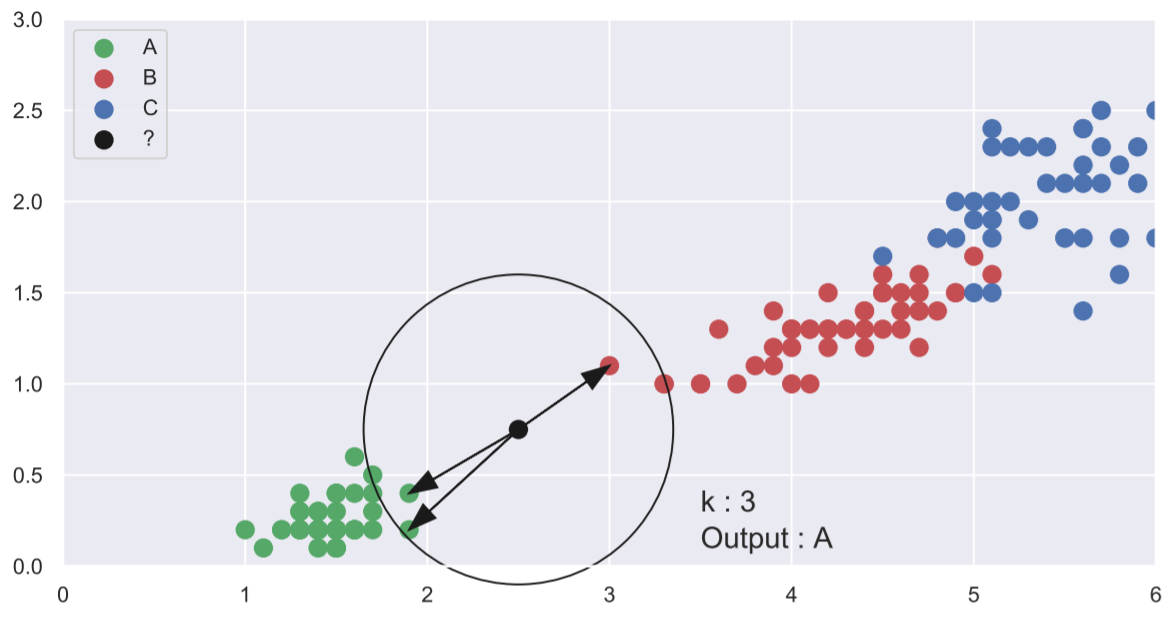
\includegraphics[width=12cm,keepaspectratio]{figs/knn_exemplo.png}
\newline \centering{ Fonte: \citeonline{tchaye2020new}}\label{fig:knn_exemplo}
\end{figure}


Analisando a Figura \ref{fig:knn_exemplo} é possível observar que, quando o valor de $k == 3$, os dois vizinhos mais próximos (maioria dentre 3) estão no \textit{cluster} à esquerda. Dessa forma, o objeto central analisado deverá receber como rótulo a classe à esquerda.

k-NN foi um dos classificadores utilizados na criação dos \textit{Stackings} apresentados neste trabalho. A métrica de distância utilizada foi a Euclidiana, onde, por exemplo, observados os elementos $A$, $B$, obtem-se os valores referentes aos eixos $x$ e $y$ (numa análise bi-dimensional) sendo que $A$ possui os valores $x_{A}$ e $y_{A}$ e $B$ possui os valores $x_{B}$ e $y_{B}$. A distância $D$ será portanto calculada como $D = \sqrt{(x_{B} - x_{A})^2 + (y_{B} - y_{A})^2}$. Ao considerar mais dimensões $n$ no espaço de parâmetros a Equação deve ser ajustada adicionando a soma dos valores $(x_{n} + y_{n})^2$ à raíz quadrada. Os valores de $k$ testados foram estipulados em um laço de repetição variando de 3 a 9 onde o melhor $k$ no intervalo $\{3, 5, 7, 9\}$ foi escolhido para cada um dos testes.


Nos experimentos apresentados nesta pesquisa o método ``\textit{KNeighborsClassifier}'' foi usado  para aplicação do k-NN e foi implementado por meio da biblioteca ``\textit{scikit-learn}'' na linguagem Python.





\subsection{MLP - \textit{Multilayer Perceptron}}
\label{nn}
Um \textit{Artificial Neural Network} é uma estrutura similar ao cérebro humano no sentido de comunicação entre os neurônios. O cérebro humano responde à estímulos nas entradas dos seus neurônios e a organização celular faz com que demais sejam ativados (ou não) em resposta ao processamento daquele estímulo. Da mesma forma, uma Rede Neural Artificial normalmente possui a quantidade de entradas correspondente ao número de \textit{features} de um \textit{dataset} a ser processado. A estrutura das demais camadas e a forma como a propagação dos estímulos acontece dependem do tipo da Rede Neural criada. A última camada de neurônios corresponde às classes dos dados analisados, de forma com que seja possível, dados os parâmetros de entrada e a propagação dos estímulos, acionar o neurônio correspondente à classe estimada.

Um perceptron, que é um tipo de Rede Neural, produz uma saída binária ao receber várias entradas. Trata-se de um modelo matemático que, ao usar uma única camada de neurônios consegue resolver apenas problemas linearmente separáveis. Por essa limitação do Perceptron de camada única, segundo \citeonline{renatotinos}, é comum se usar o Perceptron Multicamadas, uma vez que segunda camada pode combinar as saídas da primeira camada de forma a produzir uma classificação final resolvendo problemas linearmente não separáveis.

O modelo original de Perceptron foi desenvolvido por \citeonline{rosenblatt1958perceptron}, onde o autor apresentou uma arquitetura que pode ser analisada, segundo \citeonline{Goodfellow-et-al-2016}, com base na Figura \ref{fig:percep} (A):

\begin{figure}[H]
\centering
\caption{Modelos de Perceptrons. Arquitura simples (A) e multicamadas (B).}
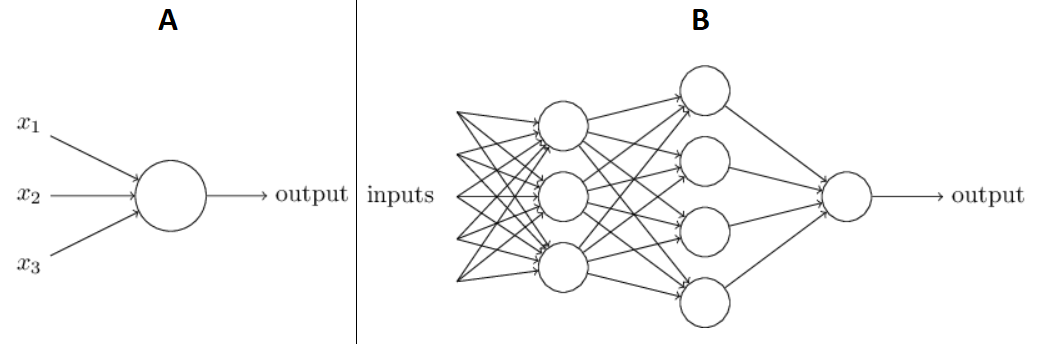
\includegraphics[width=\textwidth,keepaspectratio]{figs/perceptrons.png}
\newline\centering{ Fonte: Adaptado de \citeonline{Goodfellow-et-al-2016}.}\label{fig:percep}
\end{figure}

Para cada entrada $x_1, x_2, x_3$ introduz-se um peso $w_1, w_2, w_3$ valorados de acordo com a importância da \textit{feature} representada por cada entrada no \textit{dataset} hipotético analisado. A partir deste ponto, define-se um \textit{threshold} $t$ que será base para a saída do neurônio, sendo 0 caso a soma ponderada dos pesos para cada entrada seja menor que o valor estipulado no \textit{threshold} ($0 &\ if\ & \sum_j w_jx_j &\ \leq &\ t$) ou 1 caso o resultado seja menor ($1 &\ if\ & \sum_j w_jx_j &\ > &\ t$).

Já na Figura \ref{fig:percep} (B) é possível observar um modelo de \textit{Neural Network} (ou Perceptron com uma camada intermediária - \textit{multilayer perceptron}). Tal modelo possui a capacidade de classificação adequada a problemas de ordem mais complexa, uma vez que tal camada irá lidar com as saídas dos neurônios da primeira camada de processamento, fazendo com que o modelo seja apto a separar dados de forma não linear. Cada decisão tomada pelos neurônios da segunda camada irá ponderar as decisões tomadas na camada anterior. 

O processo de treinamento para estes tipos de redes consiste em aprender os melhores pesos (variáveis que especificam a importância de cada \textit{feature}) e bias (variável que irá balancear o \textit{threshold}). Além disso trata-se de uma rede \textit{feed-forward}, ou seja, a propagação dos dados se dá sempre no sentido das entradas para a saída. \citeonline{renatotinos} destaca que, embora seja relativamente simples, o \textit{multilayer perceptron} tem sido aplicado com sucesso como um tipo de \textit{Neural Network} na solução de vários problemas de ordem complexa.

Nos experimentos apresentados nesta pesquisa o método ``\textit{MLPClassifier}'' foi usado para criação das redes neurais e foi implementado por meio da biblioteca ``\textit{scikit-learn}'' na linguagem Python.







\subsection{SVM - \textit{Support Vector Machines}}
\label{svm}
Um classificador baseado em SVM busca, dado no espaço de parâmetros duas classes linearmente separáveis ($a$ e $b$), traçar o melhor hiperplano de forma com que o elemento da classe $a$ mais próximo ao primeiro elemento da classe $b$ sejam considerados os limites. O hiperplano, portanto, será exatamente construído na metade de tais limites. Aos limite dá-se o nome de ``vetores de suporte'' pois representam os elementos $a$ e $b$ mais próximos.

\citeonline{mueller2019aprendizado}, neste sentido, explicam que a estratégia do SVM é encontrar a maior margem de separação entre as classes, extraindo uma função de classificação para uma amostra de observações. A ideia de manter a maior margem possível para traçar o hiperplano é que as amostras de testes serão distribuídas de forma diferente no espaço de parâmetros, logo, quanto maior a margem, menor será a taxa de erro.

A Figura \ref{fig:svm} ilustra uma situação de aplicação do SVM na detecção de intrusão em redes de computadores:

\begin{figure}[H]
\centering
\caption{Exemplo de SVM.}
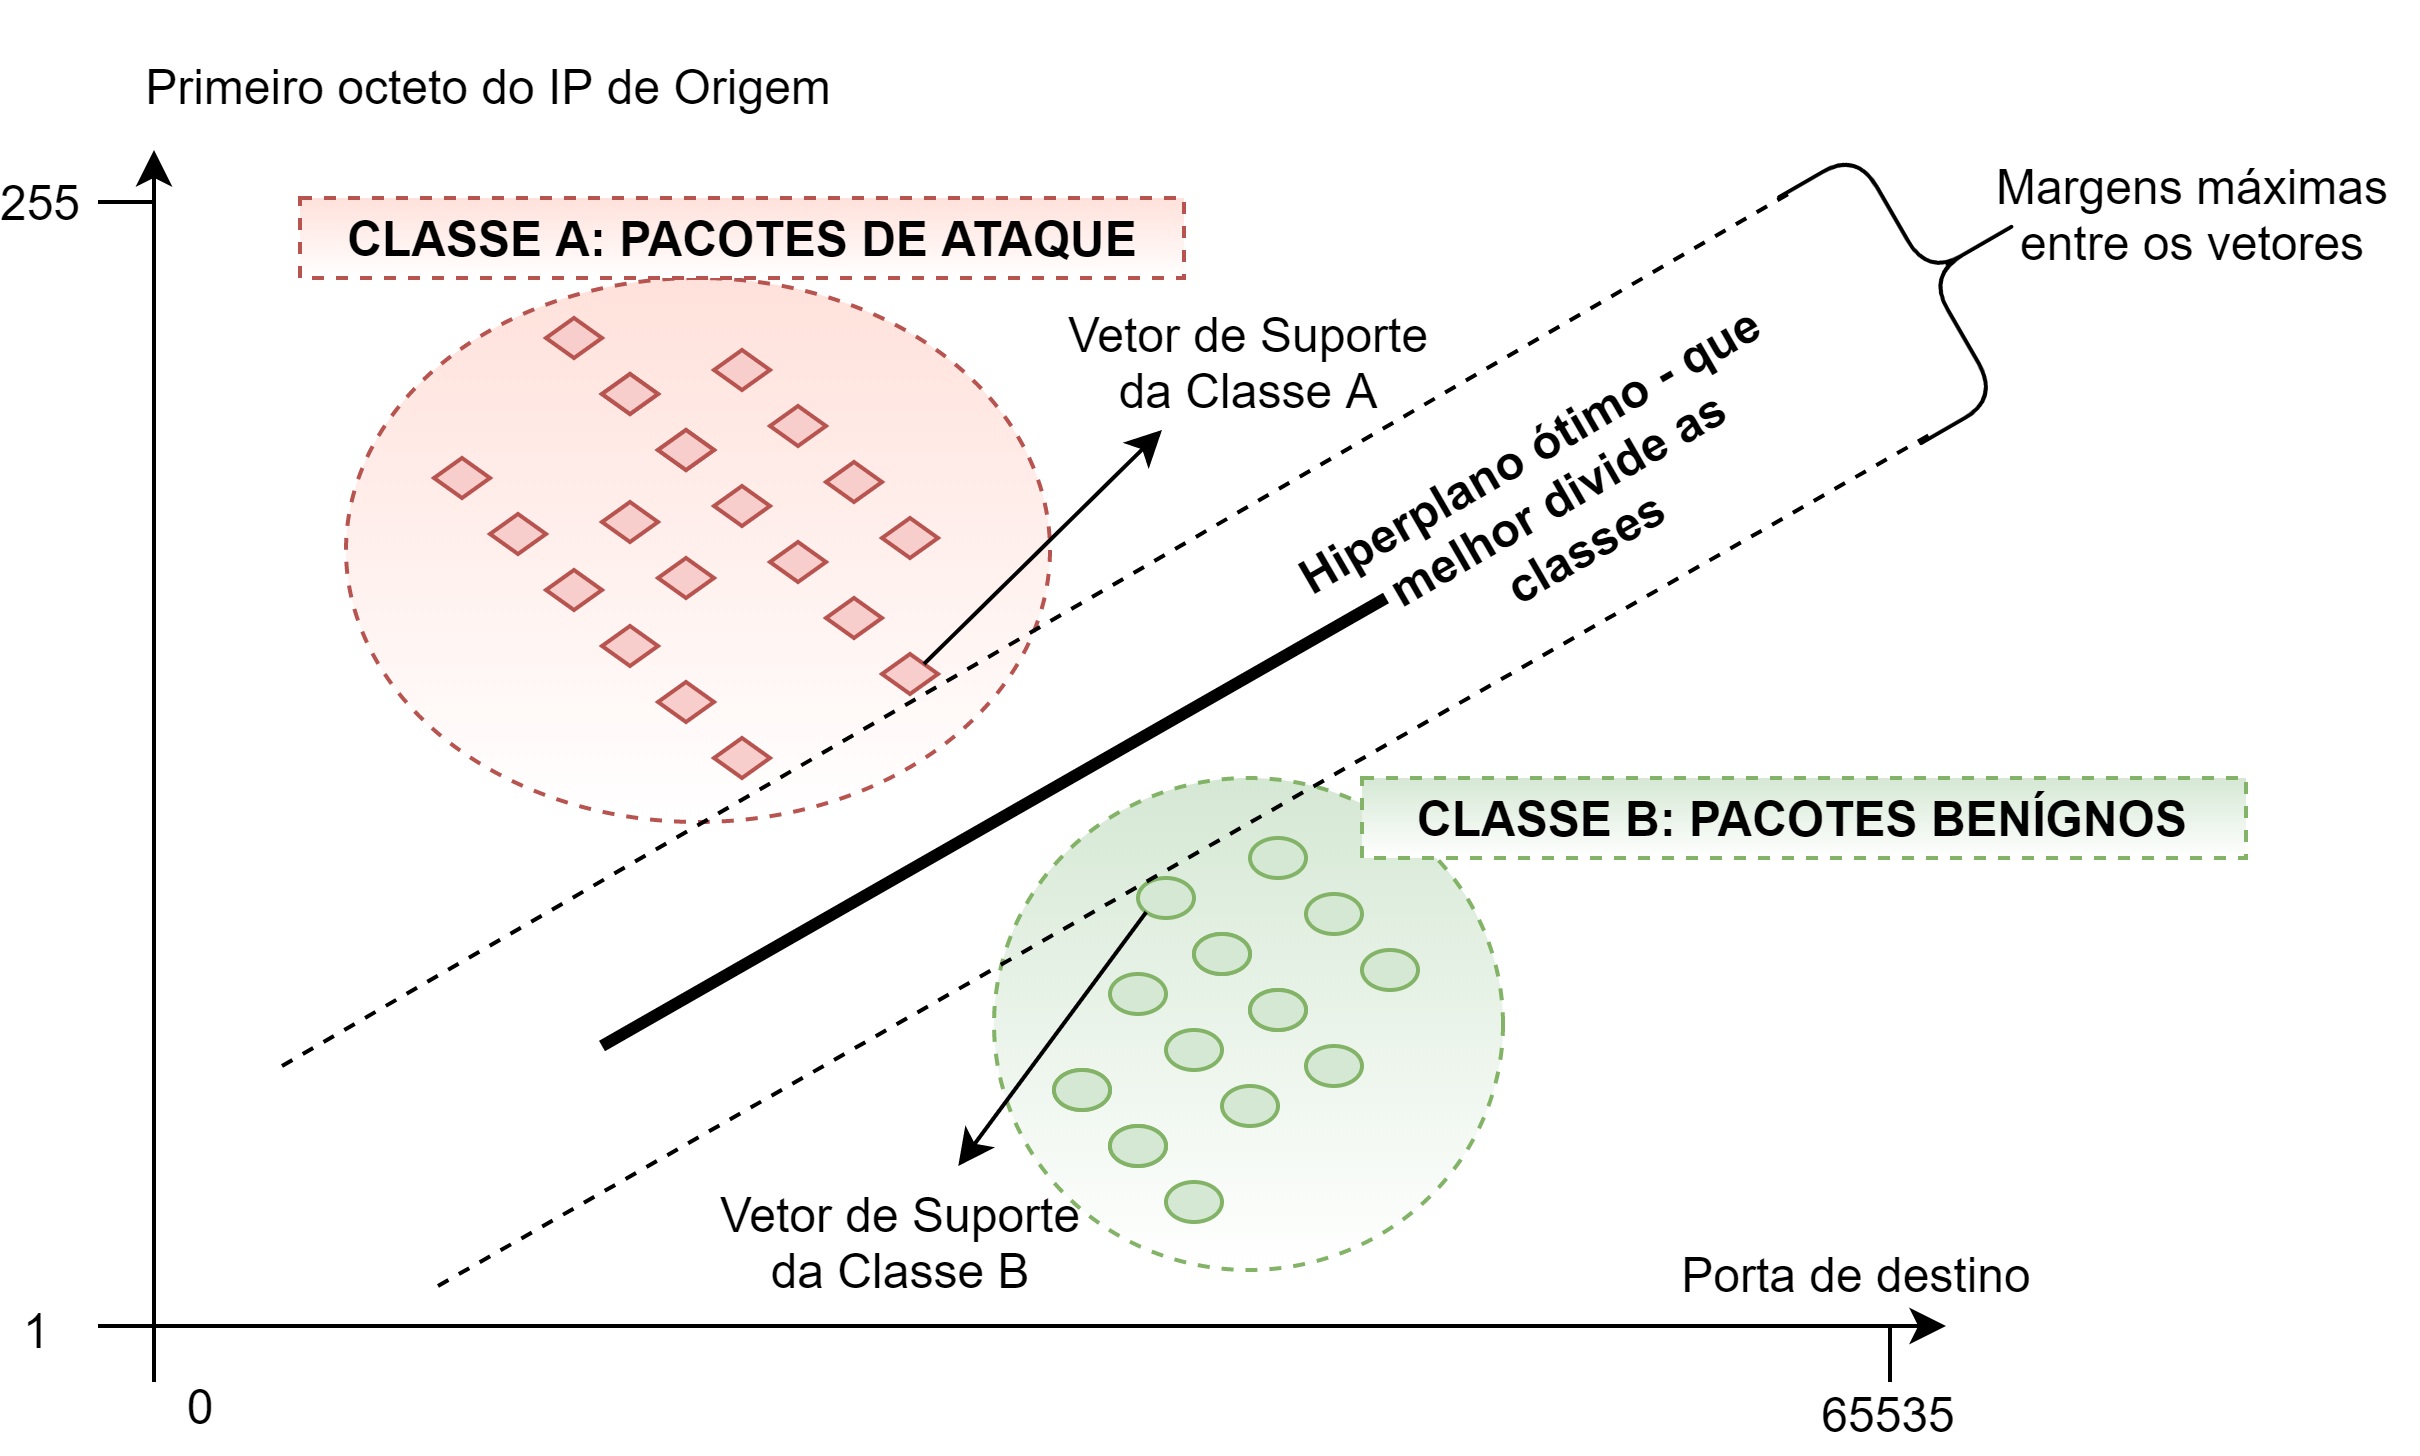
\includegraphics[width=\textwidth,keepaspectratio]{figs/svm.png}
\newline \centering{ Fonte: Elaborado pelo autor.}\label{fig:svm}
\end{figure}

Para análise da Figura \ref{fig:svm}, deve-se levar em conta que uma situação hipotética de distribuição bi-dimensional foi criada pelo autor para ilustrar o objetivo da aplicação do SVM e que, não necessariamente, apenas os parâmetros ``Primeiro octeto do IP de Origem'' (eixo $y$) e ``Porta de destino'' (eixo $x$) são úteis para classificar um tráfego de rede de maneira eficaz. 

Ademais, percebe-se que o \textit{cluster} mais à esquerda representa a ``classe A'' e todos os seus objetos onde o elemento mais próximo à ``classe B'' (situada mais à direita) é escolhido como vetor de suporte. O mesmo se aplica, em lógica inversa, a outra classe. O SVM, portanto, ao encontrar os vetores de suporte das classes analisadas estabelece as margens que representam a maior distância possível entre as classes. Por fim, um linha média entre as margens é traçada, sendo ela o hiperplano que melhor divide as classes. 


Destaca-se também a capacidade do SVM em lidar com situações de separação de classes em espaços $n$-dimensionais. No exemplo da Figura \ref{fig:svm} (supracitado para fins de compreensão do funcionamento básico do método) uma simples reta trata de dividir as classes. \citeonline{baeza2013recuperaccao} destacam que na existência de mais dimensões, o método é capaz de resolver problemas de classificação binária com igual eficácia. Se numa situação bi-dimensional a divisão das classes é realizada traçando-se uma reta, numa situação tri-dimensional, por exemplo, um plano seria desenhado de forma a realizar a classificação. Em suma, o SVM é capaz de lidar com diversas dimensões, destacando-se o custo computacional exigido à medida em que mais dimensões (e \textit{features}) são analisadas.



Nos experimentos apresentados nesta pesquisa o método ``\textit{SVC}'' foi usado para criação das \textit{Support Vector Machines} e foi implementado por meio da biblioteca ``\textit{scikit-learn}'' na linguagem Python. O kernel usado para a função de decisão do SVM foi o RBF (\textit{Radial Basis Function}).











\section{Modelagem dos \textit{Stackings}}
\label{modelagem-Stackings}
De forma a implementar os classificadores otimizados, os modelos ``clf1'', ``clf2'', ``clf3'' e ``clf4'' foram definidos de acordo com os melhores hyperparâmetros obtidos pelo processo de \textit{tune hyperparameters} descrito em \ref{subsub_hyperp}. O trecho de código na sequência escrito em Python conforme detalhes presentes no Capítulo \ref{cap-metodologia} (Metodologia) define os classificadores k-NN, MLP, DT e SVM com as configurações mais adequadas para detecção de ataques no \textit{dataset} de \textit{bruteforce}. Para os demais \textit{datasets} as diferenças estão apenas nos hyperparêmetros.

\begin{verbatim}
clf1 = KNeighborsClassifier(
          metric = 'euclidean', 
          n_neighbors = 1, 
          weights = 'uniform')
clf2 = MLPClassifier(
          max_iter = 10000,
          alpha = 0.001,
          hidden_layer_sizes = 14,
          solver = 'adam',
          random_state = 1)
clf3 = DecisionTreeClassifier(
          max_depth = 19,
          min_samples_split = 10)
clf4 = SVC(
          kernel = 'rbf',
          C=1,
          gamma=1)


\end{verbatim}



O agrupamento dos classificadores se deu inicialmente de forma exaustiva para que fosse possível obter todas as possíveis combinações. Embora este método não seja o mais adequado em se observando o tempo de processamento, ele serviu de base para a comparação entre todas as possibilidades e obtenção de um \textit{ranking} onde foi possível observar com detalhes o desempenho de todos os \textit{Ensembles}. O trecho de código na sequência define um exemplo de \textit{Stacking}:

\begin{verbatim}

stack = StackingClassifier(
           [clf1, clf2, clf4],
           meta_classifier=clf1)
\end{verbatim}

De forma a se obter as predições bem como a \textit{confusion matrix}, foram realizados testes por meio de validação cruzada, conforme trecho de código na sequência sendo ``X'' a relação de \textit{features}, ``y'' o vetor de rótulos (classes) e ``cv'' o número de validações cruzadas:

\begin{verbatim}

stack_pred = cross_val_predict(
                stack, X, y, cv=10)
conf_stack = confusion_matrix(
                y, stack_pred)
\end{verbatim}

   
   
   
   
   
   
   
   
   
   
   
   
   
   
   
A Tabela \ref{tab:modelos-stack} organiza a relação dos \textit{Ensembles} criados por meio de \textit{Stacking}:

\begin{longtable}{l|l|l}
\caption{Arquitetura dos \textit{Stackings} criados. Fonte: Elaborado pelo autor.}

\label{tab:modelos-stack}

\hline

\textbf{MODELO}   & \textbf{CAMADA 1 }             & \textbf{CAMADA 2} \\ \hline \hline


\textit{Stacking} \#1  & k-NN +   MLP            & k-NN \\ \hline
\textit{Stacking} \#2  & k-NN   + DT             & k-NN \\ \hline
\textit{Stacking} \#3  & k-NN + SVM              & k-NN \\ \hline
\textit{Stacking} \#4  & MLP   + DT              & k-NN \\ \hline
\textit{Stacking} \#5  & MLP + SVM               & k-NN \\ \hline
\textit{Stacking} \#6  & DT   + SVM              & k-NN \\ \hline
\textit{Stacking} \#7  & k-NN + MLP              & MLP  \\ \hline
\textit{Stacking} \#8  & k-NN   + DT             & MLP  \\ \hline
\textit{Stacking} \#9  & k-NN + SVM              & MLP  \\ \hline
\textit{Stacking} \#10 & MLP   + DT              & MLP  \\ \hline
\textit{Stacking} \#11 & MLP + SVM               & MLP  \\ \hline
\textit{Stacking} \#12 & DT   + SVM              & MLP  \\ \hline
\textit{Stacking} \#13 & k-NN + MLP              & DT   \\ \hline
\textit{Stacking} \#14 & k-NN   + DT             & DT   \\ \hline
\textit{Stacking} \#15 & k-NN + SVM              & DT   \\ \hline
\textit{Stacking} \#16 & MLP   + DT              & DT   \\ \hline
\textit{Stacking} \#17 & MLP + SVM               & DT   \\ \hline
\textit{Stacking} \#18 & DT   + SVM              & DT   \\ \hline
\textit{Stacking} \#19 & k-NN + MLP              & SVM  \\ \hline
\textit{Stacking} \#20 & k-NN   + DT             & SVM  \\ \hline
\textit{Stacking} \#21 & k-NN + SVM              & SVM  \\ \hline
\textit{Stacking} \#22 & MLP   + DT              & SVM  \\ \hline
\textit{Stacking} \#23 & MLP + SVM               & SVM  \\ \hline
\textit{Stacking} \#24 & DT   + SVM              & SVM  \\ \hline
\textit{Stacking} \#25 & k-NN + MLP + DT         & k-NN \\ \hline
\textit{Stacking} \#26 & k-NN   + MLP + SVM      & k-NN \\ \hline
\textit{Stacking} \#27 & k-NN + DT + SVM         & k-NN \\ \hline
\textit{Stacking} \#28 & MLP   + DT + SVM        & k-NN \\ \hline
\textit{Stacking} \#29 & k-NN + MLP + DT         & MLP  \\ \hline
\textit{Stacking} \#30 & k-NN   + MLP + SVM      & MLP  \\ \hline
\textit{Stacking} \#31 & k-NN + DT + SVM         & MLP  \\ \hline
\textit{Stacking} \#32 & MLP   + DT + SVM        & MLP  \\ \hline
\textit{Stacking} \#33 & k-NN + MLP + DT         & DT   \\ \hline
\textit{Stacking} \#34 & k-NN   + MLP + SVM      & DT   \\ \hline
\textit{Stacking} \#35 & k-NN + DT + SVM         & DT   \\ \hline
\textit{Stacking} \#36 & MLP   + DT + SVM        & DT   \\ \hline
\textit{Stacking} \#37 & k-NN + MLP + DT         & SVM  \\ \hline
\textit{Stacking} \#38 & k-NN   + MLP + SVM      & SVM  \\ \hline
\textit{Stacking} \#39 & k-NN + DT + SVM         & SVM  \\ \hline
\textit{Stacking} \#40 & MLP   + DT + SVM        & SVM  \\ \hline
\textit{Stacking} \#41 & k-NN + MLP + DT + SVM   & k-NN \\ \hline
\textit{Stacking} \#42 & k-NN   + MLP + DT + SVM & MLP  \\ \hline
\textit{Stacking} \#43 & k-NN + MLP + DT + SVM   & DT   \\ \hline
\textit{Stacking} \#44 & k-NN   + MLP + DT + SVM & SVM  \\ \hline

\end{longtable}









A Tabela \ref{tab:tempos-stack} contém a relação de tempo (custo computacional) despendido para o método exaustivo de criação dos \textit{Ensembles}. É possível observar a inviabilidade prática da utilização deste método por conta do alto tempo necessário, o que reforça ainda mais a aplicação do método de seleção de classificadores por meio da combinação baseada na \textit{Agreement Matrix} que é a proposta central desta dissertação. O hardware utilizado nos testes tinha as seguintes características: 8 processadores Intel(R) Core(TM) i7 CPU 960  @3.20GHz e 16 GB de Memória RAM. 

\begin{longtable}{l|l|l}
\caption{Tempo de processamento dedicado a criação dos \textit{Stackings} por meio de exaustão. Fonte: Elaborado pelo autor.}

\label{tab:tempos-stack}

\hline

\textbf{DATASET}   & \textbf{SEGUNDOS}             & \textbf{HORAS} \\ \hline \hline

\textit{Bruteforce} &
265145	& 73.6 \\ \hline


\textit{Infiltration} &
62527	& 17.3 \\ \hline


DDoS &
361117	& 100.3 \\ \hline


\textit{Portscan} &
415095 & 	115.3\ \hline


\textit{Botnet} &
67429	& 18.3 \\ \hline


Web &
104576	& 29.04 \\ \hline


\end{longtable}
   
   
De forma a obter uma escolha mais adequada tanto em termos de custo computacional quanto de desempenho na classificação, esta dissertação propõe uma escolha dos classificadores que comporão o \textit{Ensemble} por meio de duas análises, sendo a primeira um \textit{ranking} por AUC e a segunda a aplicação da \textit{Agreement Matrix}. Mais detalhes acerca desta proposta podem ser observados no ítem ``Q'' feito a partir da análise da Figura \ref{fig:metodologia} descrito na sequência:







A fim de resumir o processo metodológico adotado neste trabalho para a concepção dos modelos de IDS, a Figura \ref{fig:metodologia} ilustra as todas as etapas percorridas para a obtenção dos \textit{Stackings} e compilação dos resultados. 

\begin{figure}[H]
\centering
\caption{Metodologia - Visão geral do processo.}
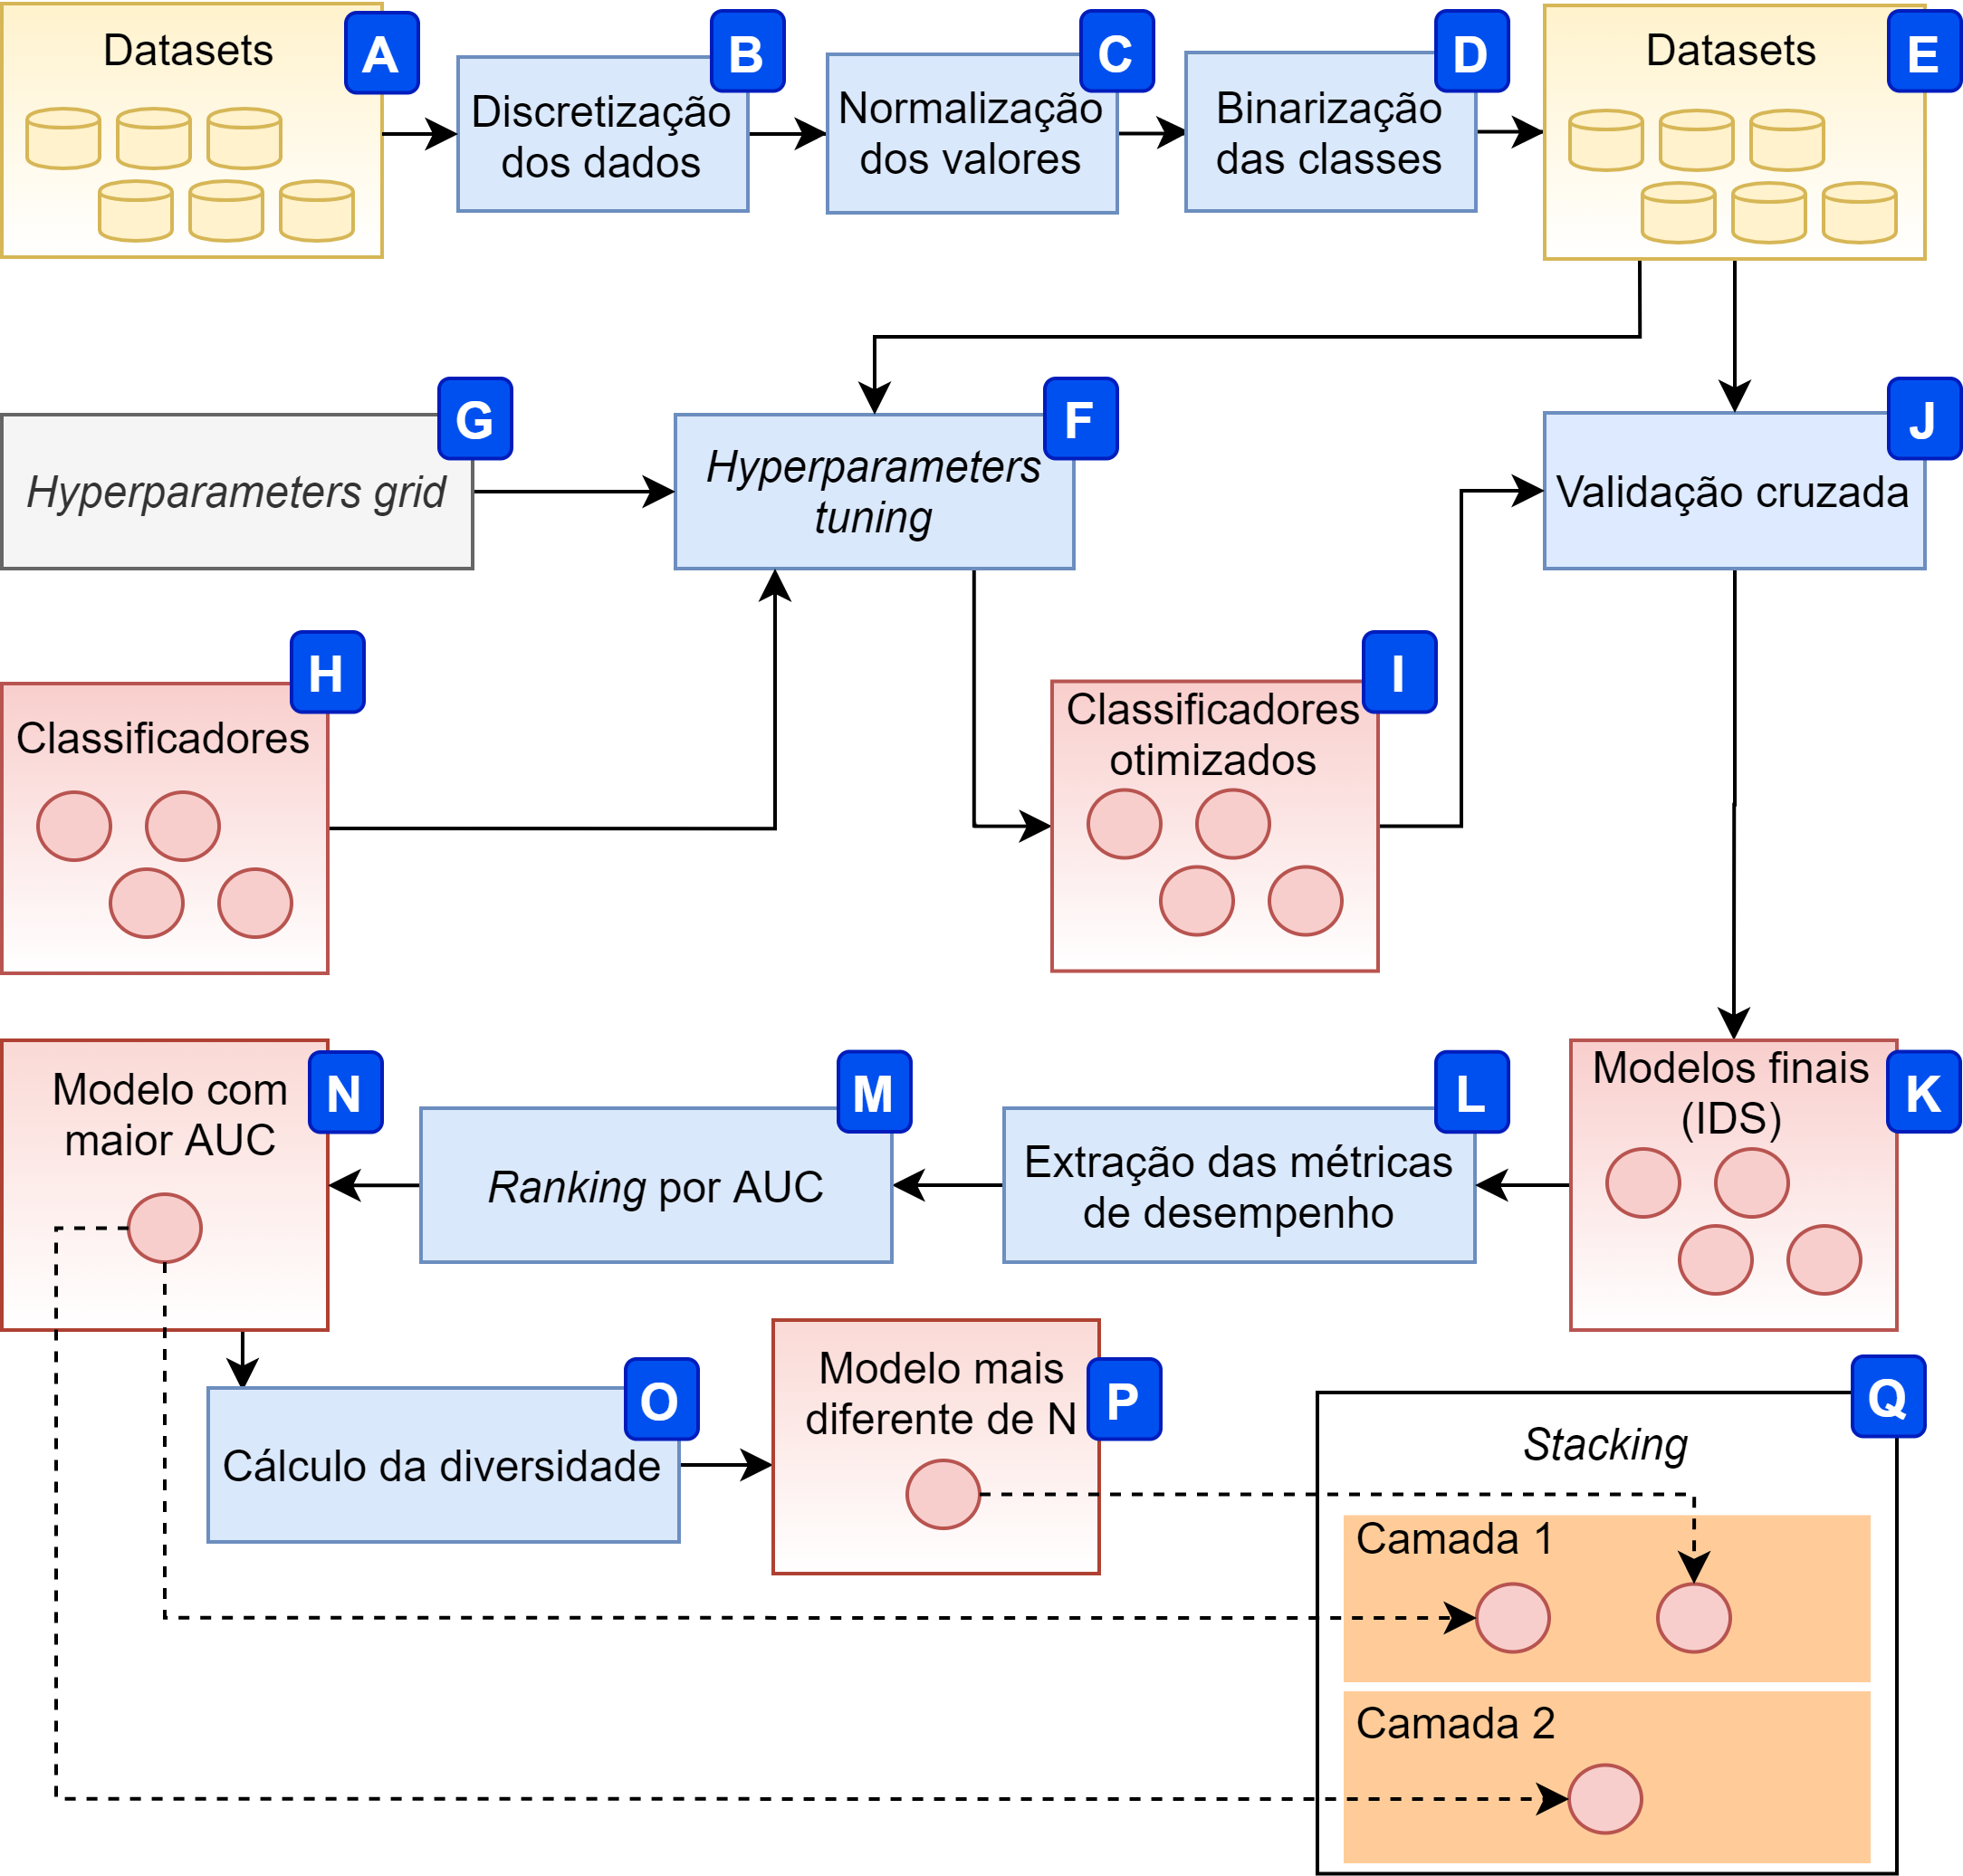
\includegraphics[width=\textwidth,keepaspectratio]{figs/metodologiafinal.png}
\newline \centering{ Fonte: Elaborado pelo autor.}\label{fig:metodologia}
\end{figure}


\subsubsection*{Metodologia - etapa ``A''}

Supracitado na Seção \ref{secao-datasets}, tratou-se do processo de obtenção dos dados para treinamento e testes considerando os dados brutos, ainda sem discretização, normalização e binarização das classes.

\subsubsection*{Metodologia - etapas ``B'', ``C'', ``D'' e ``E''}

Processos descritos anteriormente na Seção \ref{pre-processamento}. Foram relevantes para adequação dos dados aos padrões necessários de entrada de dados para os métodos de criação dos classificadores pelos algoritmos de \textit{machine learning}. 

Tais etapas que consistiram em (``B'') tranformar todos os dados em números mantendo-se a proporcionalidade das \textit{features}; (``C'') adequar os dados numéricos num mesmo intervalo de forma a garantir a não influência negativa de determinada(s) \textit{feature(s)} em específico; (``D'') criação de duas classes para garantir o objetivo principal de um detector de intrusão (que é mais detectar os ataques do que detectar o tipo deles) e (``E'') representando os dados pré-processados já adequados para a criação dos modelos classificadores e dos testes para extração das métricas de desempenho.

\subsubsection*{Metodologia - etapas ``F'', ``G'', ``H'' e ``I''}
\label{subsub_hyperp}
A utilização de métodos para obtenção dos melhores hyperparâmetros permitem criar modelos mais adequados de classificação em termos de desempenho nas taxas de detecção. 

Tratou-se de um processo de repetição onde foram testados diversos hyperparâmetros para os diferentes classificadores. A relação dos melhores valores encontrados para cada um dos \textit{datasets} podem ser observados na Tabelas \ref{tab:hyper_knn}, \ref{tab:hyper_mlp}, \ref{tab:hyper_dt} e \ref{tab:hyper_svm}:


\begin{longtable}{l|l|l|l}

\caption{Relação dos melhores hyperparâmetros para o classificador k-NN dentre todos os \textit{datasets} testados. Fonte: Elaborado pelo autor.}

\label{tab:hyper_knn}

\hline

\textbf{DATASET} & \textbf{METRIC} 		& \textbf{N\_NEIGHBORS} & \textbf{DISTANCE}        \\ \hline \hline
\textit{Bruteforce}   & \textit{euclidean} & 1  & \textit{uniform}  \\ \hline
\textit{Infiltration} & \textit{euclidean} & 7  & \textit{distance} \\ \hline
DDoS         & \textit{manhattan} & 1  & \textit{uniform}  \\ \hline
\textit{Portscan}     & \textit{manhattan} & 1  & \textit{uniform}  \\ \hline
\textit{Botnet}       & \textit{manhattan} & 21 & \textit{distance} \\ \hline
Web          & \textit{manhattan} & 21 & \textit{distance} \\ \hline

\end{longtable}












\begin{longtable}{l|l|l|l|l}
\caption{Relação dos melhores hyperparâmetros para o classificador MLP dentre todos os \textit{datasets} testados. Fonte: Elaborado pelo autor.}

\label{tab:hyper_mlp}

\hline


\textbf{DATASET} & \textbf{ALPHA} & \textbf{HIDDEN LAYERS SIZE}  & \textbf{SOLVER} & \textbf{RSTATE}         \\ \hline \hline

\textit{Bruteforce}   & 0.001     & 14 & adam   & 1 \\ \hline
\textit{Infiltration} & 0.1       & 10 & lbfgs  & 0 \\ \hline
DDoS         & 0.001     & 12 & adam   & 3 \\ \hline
\textit{Portscan}     & 0.001     & 10 & adam   & 7 \\ \hline
\textit{Botnet}       & 0.001     & 11 & adam   & 1 \\ \hline
Web          & 0.001     & 14 & adam   & 7 \\ \hline

\end{longtable}






















\begin{longtable}{l|l|l}
\caption{Relação dos melhores hyperparâmetros para o classificador DT dentre todos os \textit{datasets} testados. Fonte: Elaborado pelo autor.}

\label{tab:hyper_dt}

\hline


\textbf{DATASET} & \textbf{MAX\_DEPTH} & \textbf{MIN\_SAMPLES\_SPLIT}  \\ \hline \hline


\endfirsthead \caption[]{Continuação.} \endhead \caption[]{Fim.} \endlastfoot


\textit{Bruteforce}   & 19      & 10 \\ \hline
\textit{Infiltration} & 5       & 150 \\ \hline
DDoS         & 19      & 10 \\ \hline
\textit{Portscan}     & 13      & 10 \\ \hline
\textit{Botnet}       & 19      & 10 \\ \hline
Web          & 9       & 10 \\ \hline

\end{longtable}











\begin{longtable}{l|l|l|l}
\caption{Relação dos melhores hyperparâmetros para o classificador SVM dentre todos os \textit{datasets} testados. Fonte: Elaborado pelo autor.}

\label{tab:hyper_svm}

\hline


\textbf{DATASET} & \textbf{KERNEL} & \textbf{C} & \textbf{GAMMA}  \\ \hline \hline

\textit{Bruteforce}   & RBF & 1 & 1\\ \hline
\textit{Infiltration} & RBF & 0.01 & 0.01\\ \hline
DDoS         &  RBF & 1 & 1\\ \hline
\textit{Portscan}     & RBF & 1 & 1 \\ \hline
\textit{Botnet}       & RBF & 1 & 1 \\ \hline
Web          & RBF & 1 & 1 \\ \hline

\end{longtable}

Para que os valores supracitados fossem encontrados, uma relação de possíveis hyperparamêtros foi criada (``G'') e os classificadores (``H'') foram treinados/testados por meio de validação cruzada (``J'') nos \textit{datasets} (``E''). Os melhores desempenhos foram adotados para a relação de melhores hyperparâmetros dentre os testados de forma a gerar os classificadores otimizados (``I''). 


\subsubsection*{Metodologia - etapas ``K'' e ``L''}

Cada um dos quatro modelos otimizados (``I'') foi aplicado em cada um dos seis \textit{datasets} (``E'') de forma a gerar modelos preditivos (``K'') de onde foram possíveis extrair diversas métricas de desempenho para análise após testagem (``L''). As métricas geradas foram: acurácia (ACC), área sob a curva ROC (AUC), \textit{precision} (PREC), \textit{recall} (REC), f1-\textit{score} (F1) e os números absolutos de \textit{true positive} (TP), \textit{false positive} (FP), \textit{false negative} (FN) e \textit{true negative} (TN). Tais métrica foram abordadas em \ref{sub-metricas} (``Métricas de desempenho - visualização dos resultados'').


\subsubsection*{Metodologia - etapas ``M'', ``N'', ``O'', ``P'' e ``Q'', }

Embora o método por exaustão tenha sido aplicado para gerar todas as possíveis combinações dados os quatro classificadores e os seis \textit{datasets}, foi-se necessário criar uma lógica de forma com que a criação dos \textit{Ensembles} fosse automatizada buscando sempre criá-los observando-se a diminuição do tempo de processamento e o aumento de desempenho na classificação. A sistemática que conseguiu automatizar o processo de modelagem dos \textit{Stackings} com sucesso foi:

\begin{description}
  \item[M] - Ordena-se, da maior para a menor AUC, todos os classificadores;
  \item[N] - Obtém-se o melhor classificador $c$ em termos de AUC;
  \item[O] - Observa-se na \textit{Disagreement Measure} (supracitada em \ref{disagree}) quais os \textit{scores} de diferença na comparação entre os classificadores.   O trecho de código disponibilizado no Apêndice \ref{apendice_diversidade}, implementado em Python, foi usado para implementar a Equação \ref{eq-disagree} que calcula o valor $Q$ de diferença entre os classificadores em análise \textit{pair-wise} supracitada na Subseção \ref{disagree}
  
  As Tabelas \ref{tab:diversidade_bruteforce}, \ref{tab:diversidade_infiltration}, \ref{tab:diversidade_ddos}, \ref{tab:diversidade_portscan}, \ref{tab:diversidade_botnets} e \ref{tab:diversidade_web} disponibilizadas na sequência, documentam todos os \textit{scores} possíveis na combinação entre os classificadores para cada um dos seis \textit{datasets} analisados:





% DIVERSIDADE - BRUTEFORCE

\begin{longtable}{l|l|l}
\caption{Valores de diversidade na comparação dos classificadores para ataques de \textit{bruteforce}. Fonte: Elaborado pelo autor.}

\label{tab:diversidade_bruteforce}

\hline


\textbf{CLASSIFICADOR ``A''} & \textbf{CLASSIFICADOR ``B''} 		& \textbf{SCORE}         \\ \hline \hline

k-NN & MLP & 0.00230677 \\ \hline
k-NN & DT  & 0.00030966 \\ \hline
k-NN & SVM & 0.00525531 \\ \hline
MLP  & DT  & 0.00240101 \\ \hline
MLP  & SVM & 0.00320883 \\ \hline
\textbf{DT}   & \textbf{SVM} & \textbf{0.00531365} \\ \hline


\end{longtable}








% DIVERSIDADE - INFILTRATION

\begin{longtable}{l|l|l}
\caption{Valores de diversidade na comparação dos classificadores para ataques de \textit{infiltration}. Fonte: Elaborado pelo autor.}

\label{tab:diversidade_infiltration}

\hline


\textbf{CLASSIFICADOR ``A''} & \textbf{CLASSIFICADOR ``B''} 		& \textbf{SCORE}         \\ \hline \hline

k-NN & MLP & $4.16^9$ \\ \hline
\textbf{k-NN} & \textbf{DT}  & \textbf{$6.24^{10}$} \\ \hline
k-NN & SVM & $4.16^9$ \\ \hline
\textbf{MLP}  & \textbf{DT}  & \textbf{$6.24^{10}$} \\ \hline
MLP  & SVM & 0 \\ \hline
\textbf{DT}   & \textbf{SVM} & \textbf{$6.24^{10}$} \\ \hline


\end{longtable}











\newpage

% DIVERSIDADE - DDOS

\begin{longtable}{l|l|l}
\caption{Valores de diversidade na comparação dos classificadores para ataques DDoS. Fonte: Elaborado pelo autor.}

\label{tab:diversidade_ddos}

\hline


\textbf{CLASSIFICADOR ``A''} & \textbf{CLASSIFICADOR ``B''} 		& \textbf{SCORE}         \\ \hline \hline




k-NN & MLP & 0.00330512 \\ \hline
k-NN & DT  & 0.00112533 \\ \hline
k-NN & SVM & 0.01246732 \\ \hline
MLP  & DT  & 0.00324309 \\ \hline
MLP  & SVM & 0.01008373 \\ \hline
\textbf{DT}   & \textbf{SVM} & \textbf{0.01251162} \\ \hline


\end{longtable}
















% DIVERSIDADE - PORTSCAN

\begin{longtable}{l|l|l}
\caption{Valores de diversidade na comparação dos classificadores para ataques de \textit{portscan}. Fonte: Elaborado pelo autor.}

\label{tab:diversidade_portscan}

\hline


\textbf{CLASSIFICADOR ``A''} & \textbf{CLASSIFICADOR ``B''} 		& \textbf{SCORE}         \\ \hline \hline

k-NN & MLP & 0.00399166 \\ \hline
k-NN & DT  & 0.00056624 \\ \hline
k-NN & SVM & 0.00448101 \\ \hline
MLP  & DT  & 0.00405458 \\ \hline
MLP  & SVM & 0.00088082 \\ \hline
\textbf{DT}   & \textbf{SVM} & \textbf{0.00457189} \\ \hline


\end{longtable}









% DIVERSIDADE - BOTNET

\begin{longtable}{l|l|l}
\caption{Valores de diversidade na comparação dos classificadores para ataques provenientes de \textit{botnets}. Fonte: Elaborado pelo autor.}

\label{tab:diversidade_botnets}

\hline


\textbf{CLASSIFICADOR ``A''} & \textbf{CLASSIFICADOR ``B''} 		& \textbf{SCORE}         \\ \hline \hline

k-NN & MLP & 0.00269236 \\ \hline
k-NN & DT  & 0.00317427 \\ \hline
k-NN & SVM & 0.00296474\\ \hline
MLP  & DT  & 0.00463045 \\ \hline
MLP  & SVM & 0.00037714 \\ \hline
\textbf{DT}   & \textbf{SVM} & \textbf{0.00494473} \\ \hline


\end{longtable}
















% DIVERSIDADE - WEB

\begin{longtable}{l|l|l}
\caption{Valores de diversidade na comparação dos classificadores para ataques web. Fonte: Elaborado pelo autor.}

\label{tab:diversidade_web}

\hline


\textbf{CLASSIFICADOR ``A''} & \textbf{CLASSIFICADOR ``B''} 		& \textbf{SCORE}         \\ \hline \hline

\endfirsthead \caption[]{Continuação.} \endhead \caption[]{Fim.} \endlastfoot



k-NN & MLP & 0.00150384 \\ \hline
k-NN & DT  & 0.00048170 \\ \hline
\textbf{k-NN }& \textbf{SVM} & \textbf{0.01254772} \\ \hline
MLP  & DT  & 0.00163308 \\ \hline
MLP  & SVM & 0.01188979 \\ \hline
DT   & SVM & 0.01251248 \\ \hline


\end{longtable}



\item[P] - Na comparação entre os classificadores $c$ obteve-se o maior \textit{score}, que indica qual a combinação mais diferente de classificadores. Ou seja, o processo neste ponto foi capaz de fornecer a combinação de classificadores $c, d$ mais diferentes entre si, sendo $c$ o modelo com maior AUC obtido nas etapas ``M'' e ``N'' e $d$ o modelo mais diferente de $c$ de acordo com o processo ``O'' observando-se as \textit{Agreement Matrix}.

\item[Q] - Por fim, criaram-se os \textit{Stackings}, seguindo a metodologia da presente subseção. Na primeira camada foram aloacados os classificadores $c$ e $d$ e na segunda camada o classificador $c$. A relação de \textit{Ensembles} criados estão detalhados na Tabela x:

\begin{longtable}{l|l|l|l|l|l}
\caption{Relação de anatomia dos \textit{Stackings} criados pela proposta de análise de AUC e diversidade e tempo despendido para tal. Fonte: Elaborado pelo autor.}

\label{tab:tempo_criacao_camadas}

\hline


\textbf{ID}             & 
\textbf{DATASET}        & 
\textbf{CAMADA 1} 		& 
\textbf{CAMADA 2}       &
\textbf{SEGUNDOS}       &
\textbf{HORAS} \\ \hline \hline

\#1                      &
\textit{Bruteforce}     & 
k-NN, SVM               &
k-NN                    & 
8889                    & 
2.4                      \\ \hline

\#2                      &
\textit{Infiltration}     & 
k-NN, DT               &
k-NN                    & 
291                    & 
0.08                      \\ \hline

\#3                      &
DDoS     & 
DT, SVM               &
DT                   & 
15761                    & 
4.3                      \\ \hline

\#4                      &
\textit{Portscan}     & 
DT, SVM               &
DT                   & 
19912                    & 
5.5                      \\ \hline

\#5                      &
\textit{Botnet}     & 
DT, SVM               &
DT                   & 
684                    & 
0.19                      \\ \hline

\#6                      &
Web    & 
k-NN, SVM               &
k-NN                    & 
2272                    & 
0.6                      \\ \hline


\end{longtable}


\end{description}

No Capítulo \ref{result} são apresentados os resultados obtidos para os testes realizados.

\chapter{Resultados}
\label{result}



% DEFESA






Após a execução dos treinamentos e dos testes para cada um dos modelos criados, compilou-se os resultados de acurácia (ACC), área sob a curva ROC (AUC), \textit{precision} (PREC), \textit{recall} (REC), F1-Score (F1) e os números totais de \textit{True Positive} (TP), \textit{False Positive} (FP), \textit{False Negative} (FN) e \textit{True Negative} (TN) a fim de organizar as Tabelas \ref{tab:resultados_ind_infiltration}, \ref{tab:resultados_ind_ddos}, \ref{tab:resultados_ind_portscan}, \ref{tab:resultados_ind_botnets}, \ref{tab:resultados_ind_web} e \ref{tab:resultados_ind_bruteforce} para compilação dos resultados para os métodos individuais e a Tabelas \ref{tab:resultados_ex_bruteforce}, \ref{tab:resultados_ex_infiltration}, \ref{tab:resultados_ex_ddos}, \ref{tab:resultados_ex_portscan}, \ref{tab:resultados_ex_botnets} e \ref{tab:resultados_ex_web} para visualização do desempenho de cada um dos \textit{Stackings}:

% TABELA DOS RESULTADOS







% bruteforce

\begin{longtable}{l|l|l|l|l|l|l|l|l|l}
\caption{Resultados para os classificadores individuais na detecção de ataques de \textit{bruteforce} ordenados da maior para a menor Área sob a Curva (AUC). Fonte: Elaborado pelo autor.}
\label{tab:resultados_ind_bruteforce}

\hline

\textbf{CLF} & \textbf{ACC} 		& \textbf{AUC}      & \textbf{PREC} 	 & \textbf{REC}            & \textbf{F1}       & \textbf{TP}   & \textbf{FP} & \textbf{FN}   & \textbf{TN}     \\ \hline \hline
k-NN 		& 0.999825 	& 0.998872 & 0.99993  	 & 0.999889	  & 0.99991  & 6981 & 15 & 24   & 215802 \\ \hline
DT  		& 0.999704 	& 0.998049 & 0.99988  	 & 0.999815 	  & 0.99984 & 6970 & 26 & 40   & 215786 \\ \hline
MLP 		& 0.997653 	& 0.994501 & 0.999712 	 & 0.997864 	  & 0.99878 & 6934 & 62 & 461  & 215365 \\ \hline
SVM 		& 0.994713 	& 0.993606 & 0.999753 	 & 0.994787 	  & 0.99726 & 6943 & 53 & 1125 & 214701 \\ \hline


\end{longtable}







% infiltration

\begin{longtable}{l|l|l|l|l|l|l|l|l|l}
\caption{Resultados para os classificadores individuais na detecção de ataques de \textit{infiltration} ordenados da maior para a menor Área sob a Curva (AUC). Fonte: Elaborado pelo autor.}

\label{tab:resultados_ind_infiltration}

\hline


\textbf{CLF} & \textbf{ACC} 		& \textbf{AUC}      & \textbf{PREC} 	 & \textbf{REC}            & \textbf{F1}       & \textbf{TP}   & \textbf{FP} & \textbf{FN}   & \textbf{TN}     \\ \hline \hline
k-NN & 0.99991  & 0.657895 & 0.99991  & 1        & 0.999955 & 6 & 13 & 0 & 144178 \\ \hline
DT  & 0.999889 & 0.657884  & 0.99991  & 0.999979 & 0.999945 & 6 & 13 & 3 & 144175 \\ \hline
MLP & 0.999868 & 0.5       & 0.999868 & 1        & 0.999934 & 0 & 19 & 0 & 144178 \\ \hline
SVM & 0.999868 & 0.5       & 0.999868 & 1        & 0.999934 & 0 & 19 & 0 & 144178 \\ \hline


\end{longtable}













%ddos
\begin{longtable}{l|l|l|l|l|l|l|l|l|l}
\caption{Resultados para os classificadores individuais na detecção de ataques DDoS ordenados da maior para a menor Área sob a Curva (AUC). Fonte: Elaborado pelo autor.}

\label{tab:resultados_ind_ddos}

\hline


\textbf{CLF} & \textbf{ACC} 		& \textbf{AUC}      & \textbf{PREC} 	 & \textbf{REC}            & \textbf{F1}       & \textbf{TP}   & \textbf{FP} & \textbf{FN}   & \textbf{TN}     \\ \hline \hline

DT   & 0.999468 & 0.999466 & 0.999324 & 0.999447 & 0.999386 & 63977 & 33  & 27   & 48818 \\ \hline
k-NN & 0.99914  & 0.999073 & 0.999447 & 0.998567 & 0.999007 & 63983 & 27  & 70   & 48775 \\ \hline
MLP  & 0.996757 & 0.996532 & 0.997639 & 0.994861 & 0.996248 & 63895 & 115 & 251  & 48594 \\ \hline
SVM  & 0.987417 & 0.985792 & 0.99717  & 0.973692 & 0.985291 & 63875 & 135 & 1285 & 47560 \\ \hline
\end{longtable}












% portscan
\begin{longtable}{l|l|l|l|l|l|l|l|l|l}
\caption{Resultados para os classificadores individuais na detecção de ataques de \textit{portscan} ordenados da maior para a menor Área sob a Curva (AUC). Fonte: Elaborado pelo autor.}

\label{tab:resultados_ind_portscan}

\hline


\textbf{CLF} & \textbf{ACC} 		& \textbf{AUC}      & \textbf{PREC} 	 & \textbf{REC}            & \textbf{F1}       & \textbf{TP}   & \textbf{FP} & \textbf{FN}   & \textbf{TN}     \\ \hline \hline

DT   & 0.999692 & 0.9997   & 0.999544 & 0.999764 & 0.999654 & 79404 & 29  & 15  & 63600 \\ \hline
k-NN & 0.99956  & 0.999546 & 0.999591 & 0.999418 & 0.999505 & 79407 & 26  & 37  & 63578 \\ \hline
MLP  & 0.995917 & 0.995735 & 0.996722 & 0.994089 & 0.995404 & 79225 & 208 & 376 & 63239 \\ \hline
SVM  & 0.995358 & 0.995124 & 0.996545 & 0.993005 & 0.994772 & 79214 & 219 & 445 & 63170 \\ \hline
\end{longtable}













% botnet
\begin{longtable}{l|l|l|l|l|l|l|l|l|l}
\caption{Resultados para os classificadores individuais na detecção de ataques provenientes de \textit{botnets} ordenados da maior para a menor Área sob a Curva (AUC). Fonte: Elaborado pelo autor.}

\label{tab:resultados_ind_botnets}

\hline


\textbf{CLF} & \textbf{ACC} 		& \textbf{AUC}      & \textbf{PREC} 	 & \textbf{REC}            & \textbf{F1}       & \textbf{TP}   & \textbf{FP} & \textbf{FN}   & \textbf{TN}     \\ \hline \hline

DT    & 0.997905 & 0.951513 & 0.998994 & 0.998888 & 0.998941 & 896 & 95  & 105 & 94359 \\ \hline
MLP   & 0.995516 & 0.796038 & 0.99574  & 0.999746 & 0.997739 & 587 & 404 & 24  & 94440 \\ \hline
k-NN  & 0.997182 & 0.890239 & 0.997707 & 0.99945  & 0.998577 & 774 & 217 & 52  & 94412 \\ \hline
SVM   & 0.995223 & 0.780913 & 0.995426 & 0.999767 & 0.997592 & 557 & 434 & 22  & 94442 \\ \hline
\end{longtable}










%web
\begin{longtable}{l|l|l|l|l|l|l|l|l|l}
\caption{Resultados para os classificadores individuais na detecção de ataques web ordenados da maior para a menor Área sob a Curva (AUC). Fonte: Elaborado pelo autor.}

\label{tab:resultados_ind_web}

\hline


\textbf{CLF} & \textbf{ACC} 		& \textbf{AUC}      & \textbf{PREC} 	 & \textbf{REC}            & \textbf{F1}       & \textbf{TP}   & \textbf{FP} & \textbf{FN}   & \textbf{TN}     \\ \hline \hline

k-NN & 0.999683 & 0.993489 & 0.999833 & 0.999845 & 0.999839 & 1074 & 14   & 13 & 84014 \\ \hline
DT   & 0.999507 & 0.989317 & 0.999726 & 0.999774 & 0.99975  & 1065 & 23   & 19 & 84008 \\ \hline
MLP  & 0.99839  & 0.955185 & 0.998846 & 0.999524 & 0.999185 & 991  & 97   & 40 & 83987 \\ \hline
SVM  & 0.987441 & 0.509185 & 0.987449 & 0.999988 & 0.993679 & 20   & 1068 & 1  & 84026 \\ \hline
\end{longtable}

Embora o método de exaustão (criar todas as possíveis combinações de \textit{Stackings} dados os quatro classificadores escolhidos) não seja o mais adequado por questões de custo computacional, seus resultados permitem uma comparação de desempenho entre todas as possibilidade de \textit{Ensemble}. Ademais, por meio de análise empírica, foi possível chegar a conclusão de que a melhor forma de criar os \textit{committees} era observando a relação AUC e diversidade. As Tabelas \ref{tab:resultados_ex_bruteforce}, \ref{tab:resultados_ex_infiltration}, \ref{tab:resultados_ex_ddos}, \ref{tab:resultados_ex_portscan}, \ref{tab:resultados_ex_botnets} e \ref{tab:resultados_ex_web} documentam todos os resultados obtidos por exaustão:



% TABELA DOS RESULTADOS EXAUSTAO

\begin{longtable}{l|l|l|l|l|l|l|l|l|l}
\caption{Resultados para os \textit{Stackings} na detecção de ataques \textit{bruteforce}. Fonte: Elaborado pelo autor.}

\label{tab:resultados_ex_bruteforce}

\hline


     \textbf{ID} & \textbf{ACC} 		& \textbf{AUC}      & \textbf{PREC} 	 & \textbf{REC}            & \textbf{F1}       & \textbf{TP}   & \textbf{FP} & \textbf{FN}   & \textbf{TN}     \\ \hline \hline 

\endfirsthead \caption[]{Continuação.} \endhead \caption[]{Fim.} \endlastfoot

\#1  & 0.999825 & 0.998872 & 0.99993  & 0.999889 & 0.99991  & 6981 & 15 & 24  & 215802 \\ \hline
\#2  & 0.999825 & 0.998872 & 0.99993  & 0.999889 & 0.99991  & 6981 & 15 & 24  & 215802 \\ \hline
\#3  & 0.999825 & 0.998872 & 0.99993  & 0.999889 & 0.99991  & 6981 & 15 & 24  & 215802 \\ \hline
\#4  & 0.999677 & 0.997897 & 0.99987  & 0.999796 & 0.999833 & 6968 & 28 & 44  & 215782 \\ \hline
\#5  & 0.997738 & 0.994476 & 0.999708 & 0.997957 & 0.998831 & 6933 & 63 & 441 & 215385 \\ \hline
\#6  & 0.999722 & 0.998128 & 0.999884 & 0.999829 & 0.999856 & 6971 & 25 & 37  & 215789 \\ \hline
\#7  & 0.999825 & 0.998872 & 0.99993  & 0.999889 & 0.99991  & 6981 & 15 & 24  & 215802 \\ \hline
\#8  & 0.999825 & 0.998872 & 0.99993  & 0.999889 & 0.99991  & 6981 & 15 & 24  & 215802 \\ \hline
\#9  & 0.999825 & 0.998872 & 0.99993  & 0.999889 & 0.99991  & 6981 & 15 & 24  & 215802 \\ \hline
\#10 & 0.999713 & 0.998123 & 0.999884 & 0.999819 & 0.999852 & 6971 & 25 & 39  & 215787 \\ \hline
\#11 & 0.997738 & 0.994476 & 0.999708 & 0.997957 & 0.998831 & 6933 & 63 & 441 & 215385 \\ \hline
\#12 & 0.999713 & 0.997985 & 0.999875 & 0.999829 & 0.999852 & 6969 & 27 & 37  & 215789 \\ \hline
\#13 & 0.999825 & 0.998872 & 0.99993  & 0.999889 & 0.99991  & 6981 & 15 & 24  & 215802 \\ \hline
\#14 & 0.999825 & 0.998872 & 0.99993  & 0.999889 & 0.99991  & 6981 & 15 & 24  & 215802 \\ \hline
\#15 & 0.999825 & 0.998872 & 0.99993  & 0.999889 & 0.99991  & 6981 & 15 & 24  & 215802 \\ \hline
\#16 & 0.999695 & 0.997906 & 0.99987  & 0.999815 & 0.999842 & 6968 & 28 & 40  & 215786 \\ \hline
\#17 & 0.997738 & 0.994476 & 0.999708 & 0.997957 & 0.998831 & 6933 & 63 & 441 & 215385 \\ \hline
\#18 & 0.99969  & 0.998042 & 0.99988  & 0.999801 & 0.99984  & 6970 & 26 & 43  & 215783 \\ \hline
\#19 & 0.999825 & 0.998872 & 0.99993  & 0.999889 & 0.99991  & 6981 & 15 & 24  & 215802 \\ \hline
\#20 & 0.999825 & 0.998872 & 0.99993  & 0.999889 & 0.99991  & 6981 & 15 & 24  & 215802 \\ \hline
\#21 & 0.999825 & 0.998872 & 0.99993  & 0.999889 & 0.99991  & 6981 & 15 & 24  & 215802 \\ \hline
\#22 & 0.999695 & 0.997837 & 0.999866 & 0.999819 & 0.999842 & 6967 & 29 & 39  & 215787 \\ \hline
\#23 & 0.997738 & 0.994476 & 0.999708 & 0.997957 & 0.998831 & 6933 & 63 & 441 & 215385 \\ \hline
\#24 & 0.999726 & 0.998061 & 0.99988  & 0.999838 & 0.999859 & 6970 & 26 & 35  & 215791 \\ \hline
\#25 & 0.99982  & 0.99887  & 0.99993  & 0.999884 & 0.999907 & 6981 & 15 & 25  & 215801 \\ \hline
\#26 & 0.999825 & 0.998872 & 0.99993  & 0.999889 & 0.99991  & 6981 & 15 & 24  & 215802 \\ \hline
\#27 & 0.999798 & 0.998858 & 0.99993  & 0.999861 & 0.999896 & 6981 & 15 & 30  & 215796 \\ \hline
\#28 & 0.999699 & 0.997909 & 0.99987  & 0.999819 & 0.999845 & 6968 & 28 & 39  & 215787 \\ \hline
\#29 & 0.999825 & 0.998872 & 0.99993  & 0.999889 & 0.99991  & 6981 & 15 & 24  & 215802 \\ \hline
\#30 & 0.999825 & 0.998872 & 0.99993  & 0.999889 & 0.99991  & 6981 & 15 & 24  & 215802 \\ \hline
\#31 & 0.999847 & 0.998676 & 0.999917 & 0.999926 & 0.999921 & 6978 & 18 & 16  & 215810 \\ \hline
\#32 & 0.999717 & 0.997918 & 0.99987  & 0.999838 & 0.999854 & 6968 & 28 & 35  & 215791 \\ \hline
\#33 & 0.999825 & 0.998872 & 0.99993  & 0.999889 & 0.99991  & 6981 & 15 & 24  & 215802 \\ \hline
\#34 & 0.999825 & 0.998872 & 0.99993  & 0.999889 & 0.99991  & 6981 & 15 & 24  & 215802 \\ \hline
\#35 & 0.999825 & 0.998872 & 0.99993  & 0.999889 & 0.99991  & 6981 & 15 & 24  & 215802 \\ \hline
\#36 & 0.999722 & 0.997989 & 0.999875 & 0.999838 & 0.999856 & 6969 & 27 & 35  & 215791 \\ \hline
\#37 & 0.999825 & 0.998872 & 0.99993  & 0.999889 & 0.99991  & 6981 & 15 & 24  & 215802 \\ \hline
\#38 & 0.999825 & 0.998872 & 0.99993  & 0.999889 & 0.99991  & 6981 & 15 & 24  & 215802 \\ \hline
\#39 & 0.999825 & 0.998872 & 0.99993  & 0.999889 & 0.99991  & 6981 & 15 & 24  & 215802 \\ \hline
\#40 & 0.999708 & 0.997844 & 0.999866 & 0.999833 & 0.999849 & 6967 & 29 & 36  & 215790 \\ \hline
\#41 & 0.99982  & 0.99887  & 0.99993  & 0.999884 & 0.999907 & 6981 & 15 & 25  & 215801 \\ \hline
\#42 & 0.999834 & 0.998739 & 0.999921 & 0.999907 & 0.999914 & 6979 & 17 & 20  & 215806 \\ \hline
\#43 & 0.999825 & 0.998872 & 0.99993  & 0.999889 & 0.99991  & 6981 & 15 & 24  & 215802 \\ \hline
\#44 & 0.999825 & 0.998872 & 0.99993  & 0.999889 & 0.99991  & 6981 & 15 & 24  & 215802 \\ \hline



\end{longtable}





















\begin{longtable}{l|l|l|l|l|l|l|l|l|l}
\caption{Resultados para os \textit{Stackings} na detecção de ataques \textit{infiltration}. Fonte: Elaborado pelo autor.}

\label{tab:resultados_ex_infiltration}

\hline


\textbf{ID} & \textbf{ACC} 		& \textbf{AUC}      & \textbf{PREC} 	 & \textbf{REC}            & \textbf{F1}       & \textbf{TP}   & \textbf{FP} & \textbf{FN}   & \textbf{TN}     \\ \hline \hline 

\endfirsthead \caption[]{Continuação.} \endhead \caption[]{Fim.} \endlastfoot

\#1  & 0.99991  & 0.657895 & 0.99991  & 1        & 0.999955 & 6 & 13 & 0 & 144178 \\ \hline
\#2  & 0.999917 & 0.710523 & 0.999924 & 0.999993 & 0.999958 & 8 & 11 & 1 & 144177 \\ \hline
\#3  & 0.99991  & 0.657895 & 0.99991  & 1        & 0.999955 & 6 & 13 & 0 & 144178 \\ \hline
\#4  & 0.999889 & 0.657884 & 0.99991  & 0.999979 & 0.999945 & 6 & 13 & 3 & 144175 \\ \hline
\#5  & 0.999868 & 0.5      & 0.999868 & 1        & 0.999934 & 0 & 19 & 0 & 144178 \\ \hline
\#6  & 0.999882 & 0.657881 & 0.99991  & 0.999972 & 0.999941 & 6 & 13 & 4 & 144174 \\ \hline
\#7  & 0.99991  & 0.657895 & 0.99991  & 1        & 0.999955 & 6 & 13 & 0 & 144178 \\ \hline
\#8  & 0.999903 & 0.631579 & 0.999903 & 1        & 0.999951 & 5 & 14 & 0 & 144178 \\ \hline
\#9  & 0.99991  & 0.657895 & 0.99991  & 1        & 0.999955 & 6 & 13 & 0 & 144178 \\ \hline
\#10 & 0.999868 & 0.5      & 0.999868 & 1        & 0.999934 & 0 & 19 & 0 & 144178 \\ \hline
\#11 & 0.999868 & 0.5      & 0.999868 & 1        & 0.999934 & 0 & 19 & 0 & 144178 \\ \hline
\#12 & 0.999868 & 0.5      & 0.999868 & 1        & 0.999934 & 0 & 19 & 0 & 144178 \\ \hline
\#13 & 0.99991  & 0.657895 & 0.99991  & 1        & 0.999955 & 6 & 13 & 0 & 144178 \\ \hline
\#14 & 0.99991  & 0.657895 & 0.99991  & 1        & 0.999955 & 6 & 13 & 0 & 144178 \\ \hline
\#15 & 0.99991  & 0.657895 & 0.99991  & 1        & 0.999955 & 6 & 13 & 0 & 144178 \\ \hline
\#16 & 0.999882 & 0.657881 & 0.99991  & 0.999972 & 0.999941 & 6 & 13 & 4 & 144174 \\ \hline
\#17 & 0.999868 & 0.5      & 0.999868 & 1        & 0.999934 & 0 & 19 & 0 & 144178 \\ \hline
\#18 & 0.999882 & 0.657881 & 0.99991  & 0.999972 & 0.999941 & 6 & 13 & 4 & 144174 \\ \hline
\#19 & 0.999868 & 0.5      & 0.999868 & 1        & 0.999934 & 0 & 19 & 0 & 144178 \\ \hline
\#20 & 0.999868 & 0.5      & 0.999868 & 1        & 0.999934 & 0 & 19 & 0 & 144178 \\ \hline
\#21 & 0.999868 & 0.5      & 0.999868 & 1        & 0.999934 & 0 & 19 & 0 & 144178 \\ \hline
\#22 & 0.999868 & 0.5      & 0.999868 & 1        & 0.999934 & 0 & 19 & 0 & 144178 \\ \hline
\#23 & 0.999868 & 0.5      & 0.999868 & 1        & 0.999934 & 0 & 19 & 0 & 144178 \\ \hline
\#24 & 0.999868 & 0.5      & 0.999868 & 1        & 0.999934 & 0 & 19 & 0 & 144178 \\ \hline
\#25 & 0.99991  & 0.710519 & 0.999924 & 0.999986 & 0.999955 & 8 & 11 & 2 & 144176 \\ \hline
\#26 & 0.99991  & 0.657895 & 0.99991  & 1        & 0.999955 & 6 & 13 & 0 & 144178 \\ \hline
\#27 & 0.99991  & 0.710519 & 0.999924 & 0.999986 & 0.999955 & 8 & 11 & 2 & 144176 \\ \hline
\#28 & 0.999882 & 0.657881 & 0.99991  & 0.999972 & 0.999941 & 6 & 13 & 4 & 144174 \\ \hline
\#29 & 0.999882 & 0.552632 & 0.999882 & 1        & 0.999941 & 2 & 17 & 0 & 144178 \\ \hline
\#30 & 0.999868 & 0.5      & 0.999868 & 1        & 0.999934 & 0 & 19 & 0 & 144178 \\ \hline
\#31 & 0.999882 & 0.552632 & 0.999882 & 1        & 0.999941 & 2 & 17 & 0 & 144178 \\ \hline
\#32 & 0.999868 & 0.5      & 0.999868 & 1        & 0.999934 & 0 & 19 & 0 & 144178 \\ \hline
\#33 & 0.99991  & 0.657895 & 0.99991  & 1        & 0.999955 & 6 & 13 & 0 & 144178 \\ \hline
\#34 & 0.99991  & 0.657895 & 0.99991  & 1        & 0.999955 & 6 & 13 & 0 & 144178 \\ \hline
\#35 & 0.99991  & 0.657895 & 0.99991  & 1        & 0.999955 & 6 & 13 & 0 & 144178 \\ \hline
\#36 & 0.999889 & 0.657884 & 0.99991  & 0.999979 & 0.999945 & 6 & 13 & 3 & 144175 \\ \hline
\#37 & 0.999868 & 0.5      & 0.999868 & 1        & 0.999934 & 0 & 19 & 0 & 144178 \\ \hline
\#38 & 0.999868 & 0.5      & 0.999868 & 1        & 0.999934 & 0 & 19 & 0 & 144178 \\ \hline
\#39 & 0.999868 & 0.5      & 0.999868 & 1        & 0.999934 & 0 & 19 & 0 & 144178 \\ \hline
\#40 & 0.999868 & 0.5      & 0.999868 & 1        & 0.999934 & 0 & 19 & 0 & 144178 \\ \hline
\#41 & 0.99991  & 0.710519 & 0.999924 & 0.999986 & 0.999955 & 8 & 11 & 2 & 144176 \\ \hline
\#42 & 0.999903 & 0.657891 & 0.99991  & 0.999993 & 0.999951 & 6 & 13 & 1 & 144177 \\ \hline
\#43 & 0.99991  & 0.657895 & 0.99991  & 1        & 0.999955 & 6 & 13 & 0 & 144178 \\ \hline
\#44 & 0.999868 & 0.5      & 0.999868 & 1        & 0.999934 & 0 & 19 & 0 & 144178 \\ \hline



\end{longtable}

























\begin{longtable}{l|l|l|l|l|l|l|l|l|l}
\caption{Resultados para os \textit{Stackings} na detecção de ataques DDoS. Fonte: Elaborado pelo autor.}

\label{tab:resultados_ex_ddos}

\hline


\textbf{ID} & \textbf{ACC} 		& \textbf{AUC}      & \textbf{PREC} 	 & \textbf{REC}            & \textbf{F1}       & \textbf{TP}   & \textbf{FP} & \textbf{FN}   & \textbf{TN}     \\ \hline \hline 

\endfirsthead \caption[]{Continuação.} \endhead \caption[]{Fim.} \endlastfoot

\#1  & 0.99914  & 0.999073 & 0.999447 & 0.998567 & 0.999007 & 63983 & 27  & 70  & 48775 \\ \hline
\#2  & 0.99914  & 0.999073 & 0.999447 & 0.998567 & 0.999007 & 63983 & 27  & 70  & 48775 \\ \hline
\#3  & 0.99914  & 0.999073 & 0.999447 & 0.998567 & 0.999007 & 63983 & 27  & 70  & 48775 \\ \hline
\#4  & 0.999415 & 0.999407 & 0.999304 & 0.999345 & 0.999324 & 63976 & 34  & 32  & 48813 \\ \hline
\#5  & 0.996695 & 0.996502 & 0.997292 & 0.995066 & 0.996178 & 63878 & 132 & 241 & 48604 \\ \hline
\#6  & 0.999451 & 0.999448 & 0.999304 & 0.999427 & 0.999365 & 63976 & 34  & 28  & 48817 \\ \hline
\#7  & 0.99914  & 0.999073 & 0.999447 & 0.998567 & 0.999007 & 63983 & 27  & 70  & 48775 \\ \hline
\#8  & 0.99914  & 0.999073 & 0.999447 & 0.998567 & 0.999007 & 63983 & 27  & 70  & 48775 \\ \hline
\#9  & 0.99914  & 0.999073 & 0.999447 & 0.998567 & 0.999007 & 63983 & 27  & 70  & 48775 \\ \hline
\#10 & 0.999468 & 0.999463 & 0.999345 & 0.999427 & 0.999386 & 63978 & 32  & 28  & 48817 \\ \hline
\#11 & 0.996757 & 0.996532 & 0.997639 & 0.994861 & 0.996248 & 63895 & 115 & 251 & 48594 \\ \hline
\#12 & 0.999468 & 0.999463 & 0.999345 & 0.999427 & 0.999386 & 63978 & 32  & 28  & 48817 \\ \hline
\#13 & 0.99914  & 0.999073 & 0.999447 & 0.998567 & 0.999007 & 63983 & 27  & 70  & 48775 \\ \hline
\#14 & 0.99914  & 0.999073 & 0.999447 & 0.998567 & 0.999007 & 63983 & 27  & 70  & 48775 \\ \hline
\#15 & 0.99914  & 0.999073 & 0.999447 & 0.998567 & 0.999007 & 63983 & 27  & 70  & 48775 \\ \hline
\#16 & 0.999442 & 0.99943  & 0.999365 & 0.999345 & 0.999355 & 63979 & 31  & 32  & 48813 \\ \hline
\#17 & 0.996757 & 0.996532 & 0.997639 & 0.994861 & 0.996248 & 63895 & 115 & 251 & 48594 \\ \hline
\#18 & 0.999371 & 0.999351 & 0.999345 & 0.999202 & 0.999273 & 63978 & 32  & 39  & 48806 \\ \hline
\#19 & 0.99914  & 0.999073 & 0.999447 & 0.998567 & 0.999007 & 63983 & 27  & 70  & 48775 \\ \hline
\#20 & 0.99914  & 0.999073 & 0.999447 & 0.998567 & 0.999007 & 63983 & 27  & 70  & 48775 \\ \hline
\#21 & 0.99914  & 0.999073 & 0.999447 & 0.998567 & 0.999007 & 63983 & 27  & 70  & 48775 \\ \hline
\#22 & 0.999424 & 0.999415 & 0.999324 & 0.999345 & 0.999335 & 63977 & 33  & 32  & 48813 \\ \hline
\#23 & 0.996757 & 0.996532 & 0.997639 & 0.994861 & 0.996248 & 63895 & 115 & 251 & 48594 \\ \hline
\#24 & 0.999424 & 0.99942  & 0.999284 & 0.999386 & 0.999335 & 63975 & 35  & 30  & 48815 \\ \hline
\#25 & 0.999194 & 0.999146 & 0.999345 & 0.998792 & 0.999068 & 63978 & 32  & 59  & 48786 \\ \hline
\#26 & 0.99914  & 0.999073 & 0.999447 & 0.998567 & 0.999007 & 63983 & 27  & 70  & 48775 \\ \hline
\#27 & 0.999176 & 0.999128 & 0.999324 & 0.998772 & 0.999048 & 63977 & 33  & 60  & 48785 \\ \hline
\#28 & 0.999327 & 0.999304 & 0.999304 & 0.99914  & 0.999222 & 63976 & 34  & 42  & 48803 \\ \hline
\#29 & 0.999282 & 0.999251 & 0.999324 & 0.999017 & 0.999171 & 63977 & 33  & 48  & 48797 \\ \hline
\#30 & 0.99914  & 0.999073 & 0.999447 & 0.998567 & 0.999007 & 63983 & 27  & 70  & 48775 \\ \hline
\#31 & 0.999176 & 0.999128 & 0.999324 & 0.998772 & 0.999048 & 63977 & 33  & 60  & 48785 \\ \hline
\#32 & 0.999344 & 0.999327 & 0.999283 & 0.999202 & 0.999242 & 63975 & 35  & 39  & 48806 \\ \hline
\#33 & 0.99914  & 0.999073 & 0.999447 & 0.998567 & 0.999007 & 63983 & 27  & 70  & 48775 \\ \hline
\#34 & 0.99914  & 0.999073 & 0.999447 & 0.998567 & 0.999007 & 63983 & 27  & 70  & 48775 \\ \hline
\#35 & 0.99914  & 0.999073 & 0.999447 & 0.998567 & 0.999007 & 63983 & 27  & 70  & 48775 \\ \hline
\#36 & 0.999389 & 0.999374 & 0.999324 & 0.999263 & 0.999294 & 63977 & 33  & 36  & 48809 \\ \hline
\#37 & 0.99914  & 0.999073 & 0.999447 & 0.998567 & 0.999007 & 63983 & 27  & 70  & 48775 \\ \hline
\#38 & 0.99914  & 0.999073 & 0.999447 & 0.998567 & 0.999007 & 63983 & 27  & 70  & 48775 \\ \hline
\#39 & 0.99914  & 0.999073 & 0.999447 & 0.998567 & 0.999007 & 63983 & 27  & 70  & 48775 \\ \hline
\#40 & 0.999371 & 0.999351 & 0.999345 & 0.999202 & 0.999273 & 63978 & 32  & 39  & 48806 \\ \hline
\#41 & 0.999229 & 0.999177 & 0.999426 & 0.998792 & 0.999109 & 63982 & 28  & 59  & 48786 \\ \hline
\#42 & 0.999185 & 0.999133 & 0.999365 & 0.998751 & 0.999058 & 63979 & 31  & 61  & 48784 \\ \hline
\#43 & 0.99914  & 0.999073 & 0.999447 & 0.998567 & 0.999007 & 63983 & 27  & 70  & 48775 \\ \hline
\#44 & 0.99914  & 0.999073 & 0.999447 & 0.998567 & 0.999007 & 63983 & 27  & 70  & 48775 \\ \hline



\end{longtable}













\begin{longtable}{l|l|l|l|l|l|l|l|l|l}
\caption{Resultados para os \textit{Stackings} na detecção de ataques de \textit{portscan}. Fonte: Elaborado pelo autor.}

\label{tab:resultados_ex_portscan}

\hline


\textbf{ID} & \textbf{ACC} 		& \textbf{AUC}      & \textbf{PREC} 	 & \textbf{REC}            & \textbf{F1}       & \textbf{TP}   & \textbf{FP} & \textbf{FN}   & \textbf{TN}     \\ \hline \hline 

\endfirsthead \caption[]{Continuação.} \endhead \caption[]{Fim.} \endlastfoot

\#1  & 0.99956  & 0.999546 & 0.999591 & 0.999418 & 0.999505 & 79407 & 26  & 37  & 63578 \\ \hline
\#2  & 0.999539 & 0.999522 & 0.999591 & 0.999371 & 0.999481 & 79407 & 26  & 40  & 63575 \\ \hline
\#3  & 0.99956  & 0.999546 & 0.999591 & 0.999418 & 0.999505 & 79407 & 26  & 37  & 63578 \\ \hline
\#4  & 0.999685 & 0.999693 & 0.999529 & 0.999764 & 0.999646 & 79403 & 30  & 15  & 63600 \\ \hline
\#5  & 0.995959 & 0.995803 & 0.996519 & 0.994388 & 0.995452 & 79212 & 221 & 357 & 63258 \\ \hline
\#6  & 0.999713 & 0.999723 & 0.999544 & 0.999811 & 0.999678 & 79404 & 29  & 12  & 63603 \\ \hline
\#7  & 0.99956  & 0.999546 & 0.999591 & 0.999418 & 0.999505 & 79407 & 26  & 37  & 63578 \\ \hline
\#8  & 0.99956  & 0.999546 & 0.999591 & 0.999418 & 0.999505 & 79407 & 26  & 37  & 63578 \\ \hline
\#9  & 0.99956  & 0.999546 & 0.999591 & 0.999418 & 0.999505 & 79407 & 26  & 37  & 63578 \\ \hline
\#10 & 0.999734 & 0.999747 & 0.999544 & 0.999859 & 0.999701 & 79404 & 29  & 9   & 63606 \\ \hline
\#11 & 0.995924 & 0.995762 & 0.996534 & 0.994294 & 0.995413 & 79213 & 220 & 363 & 63252 \\ \hline
\#12 & 0.999685 & 0.999692 & 0.999544 & 0.999748 & 0.999646 & 79404 & 29  & 16  & 63599 \\ \hline
\#13 & 0.99956  & 0.999546 & 0.999591 & 0.999418 & 0.999505 & 79407 & 26  & 37  & 63578 \\ \hline
\#14 & 0.99956  & 0.999546 & 0.999591 & 0.999418 & 0.999505 & 79407 & 26  & 37  & 63578 \\ \hline
\#15 & 0.99956  & 0.999546 & 0.999591 & 0.999418 & 0.999505 & 79407 & 26  & 37  & 63578 \\ \hline
\#16 & 0.999692 & 0.9997   & 0.999544 & 0.999764 & 0.999654 & 79404 & 29  & 15  & 63600 \\ \hline
\#17 & 0.995924 & 0.995764 & 0.996518 & 0.99431  & 0.995413 & 79212 & 221 & 362 & 63253 \\ \hline
\#18 & 0.999706 & 0.999715 & 0.999544 & 0.999796 & 0.99967  & 79404 & 29  & 13  & 63602 \\ \hline
\#19 & 0.99956  & 0.999546 & 0.999591 & 0.999418 & 0.999505 & 79407 & 26  & 37  & 63578 \\ \hline
\#20 & 0.99956  & 0.999546 & 0.999591 & 0.999418 & 0.999505 & 79407 & 26  & 37  & 63578 \\ \hline
\#21 & 0.99956  & 0.999546 & 0.999591 & 0.999418 & 0.999505 & 79407 & 26  & 37  & 63578 \\ \hline
\#22 & 0.999692 & 0.9997   & 0.999544 & 0.999764 & 0.999654 & 79404 & 29  & 15  & 63600 \\ \hline
\#23 & 0.995924 & 0.995764 & 0.996518 & 0.99431  & 0.995413 & 79212 & 221 & 362 & 63253 \\ \hline
\#24 & 0.999685 & 0.999692 & 0.999544 & 0.999748 & 0.999646 & 79404 & 29  & 16  & 63599 \\ \hline
\#25 & 0.999574 & 0.999558 & 0.999623 & 0.999418 & 0.999521 & 79409 & 24  & 37  & 63578 \\ \hline
\#26 & 0.99956  & 0.999546 & 0.999591 & 0.999418 & 0.999505 & 79407 & 26  & 37  & 63578 \\ \hline
\#27 & 0.999567 & 0.99955  & 0.999623 & 0.999403 & 0.999513 & 79409 & 24  & 38  & 63577 \\ \hline
\#28 & 0.999692 & 0.999701 & 0.999529 & 0.99978  & 0.999654 & 79403 & 30  & 14  & 63601 \\ \hline
\#29 & 0.99956  & 0.999546 & 0.999591 & 0.999418 & 0.999505 & 79407 & 26  & 37  & 63578 \\ \hline
\#30 & 0.99956  & 0.999546 & 0.999591 & 0.999418 & 0.999505 & 79407 & 26  & 37  & 63578 \\ \hline
\#31 & 0.99956  & 0.999546 & 0.999591 & 0.999418 & 0.999505 & 79407 & 26  & 37  & 63578 \\ \hline
\#32 & 0.999713 & 0.999723 & 0.999544 & 0.999811 & 0.999678 & 79404 & 29  & 12  & 63603 \\ \hline
\#33 & 0.99956  & 0.999546 & 0.999591 & 0.999418 & 0.999505 & 79407 & 26  & 37  & 63578 \\ \hline
\#34 & 0.99956  & 0.999546 & 0.999591 & 0.999418 & 0.999505 & 79407 & 26  & 37  & 63578 \\ \hline
\#35 & 0.99956  & 0.999546 & 0.999591 & 0.999418 & 0.999505 & 79407 & 26  & 37  & 63578 \\ \hline
\#36 & 0.99972  & 0.999731 & 0.999544 & 0.999827 & 0.999686 & 79404 & 29  & 11  & 63604 \\ \hline
\#37 & 0.99956  & 0.999546 & 0.999591 & 0.999418 & 0.999505 & 79407 & 26  & 37  & 63578 \\ \hline
\#38 & 0.99956  & 0.999546 & 0.999591 & 0.999418 & 0.999505 & 79407 & 26  & 37  & 63578 \\ \hline
\#39 & 0.99956  & 0.999546 & 0.999591 & 0.999418 & 0.999505 & 79407 & 26  & 37  & 63578 \\ \hline
\#40 & 0.999678 & 0.999685 & 0.999529 & 0.999748 & 0.999638 & 79403 & 30  & 16  & 63599 \\ \hline
\#41 & 0.999567 & 0.99955  & 0.999623 & 0.999403 & 0.999513 & 79409 & 24  & 38  & 63577 \\ \hline
\#42 & 0.99956  & 0.999546 & 0.999591 & 0.999418 & 0.999505 & 79407 & 26  & 37  & 63578 \\ \hline
\#43 & 0.99956  & 0.999546 & 0.999591 & 0.999418 & 0.999505 & 79407 & 26  & 37  & 63578 \\ \hline
\#44 & 0.99956  & 0.999546 & 0.999591 & 0.999418 & 0.999505 & 79407 & 26  & 37  & 63578 \\ \hline


\end{longtable}




















\begin{longtable}{l|l|l|l|l|l|l|l|l|l}
\caption{Resultados para os \textit{Stackings} na detecção de ataques provenientes de \textit{botnets}. Fonte: Elaborado pelo autor.}

\label{tab:resultados_ex_botnets}

\hline


\textbf{ID} & \textbf{ACC} 		& \textbf{AUC}      & \textbf{PREC} 	 & \textbf{REC}            & \textbf{F1}       & \textbf{TP}   & \textbf{FP} & \textbf{FN}   & \textbf{TN}     \\ \hline \hline 

\endfirsthead \caption[]{Continuação.} \endhead \caption[]{Fim.} \endlastfoot

\#1  & 0.997182 & 0.890239 & 0.997707 & 0.99945  & 0.998577 & 774 & 217 & 52  & 94412 \\ \hline
\#2  & 0.997182 & 0.890239 & 0.997707 & 0.99945  & 0.998577 & 774 & 217 & 52  & 94412 \\ \hline
\#3  & 0.997182 & 0.890239 & 0.997707 & 0.99945  & 0.998577 & 774 & 217 & 52  & 94412 \\ \hline
\#4  & 0.997915 & 0.951518 & 0.998994 & 0.998899 & 0.998947 & 896 & 95  & 104 & 94360 \\ \hline
\#5  & 0.995506 & 0.796033 & 0.99574  & 0.999735 & 0.997734 & 587 & 404 & 25  & 94439 \\ \hline
\#6  & 0.99803  & 0.953074 & 0.999026 & 0.998984 & 0.999005 & 899 & 92  & 96  & 94368 \\ \hline
\#7  & 0.997182 & 0.890239 & 0.997707 & 0.99945  & 0.998577 & 774 & 217 & 52  & 94412 \\ \hline
\#8  & 0.997182 & 0.890239 & 0.997707 & 0.99945  & 0.998577 & 774 & 217 & 52  & 94412 \\ \hline
\#9  & 0.997182 & 0.890239 & 0.997707 & 0.99945  & 0.998577 & 774 & 217 & 52  & 94412 \\ \hline
\#10 & 0.997947 & 0.951534 & 0.998994 & 0.998931 & 0.998963 & 896 & 95  & 101 & 94363 \\ \hline
\#11 & 0.995506 & 0.795534 & 0.99573  & 0.999746 & 0.997734 & 586 & 405 & 24  & 94440 \\ \hline
\#12 & 0.997968 & 0.953042 & 0.999026 & 0.99892  & 0.998973 & 899 & 92  & 102 & 94362 \\ \hline
\#13 & 0.997182 & 0.890239 & 0.997707 & 0.99945  & 0.998577 & 774 & 217 & 52  & 94412 \\ \hline
\#14 & 0.997182 & 0.890239 & 0.997707 & 0.99945  & 0.998577 & 774 & 217 & 52  & 94412 \\ \hline
\#15 & 0.997182 & 0.890239 & 0.997707 & 0.99945  & 0.998577 & 774 & 217 & 52  & 94412 \\ \hline
\#16 & 0.997905 & 0.951513 & 0.998994 & 0.998888 & 0.998941 & 896 & 95  & 105 & 94359 \\ \hline
\#17 & 0.995516 & 0.796038 & 0.99574  & 0.999746 & 0.997739 & 587 & 404 & 24  & 94440 \\ \hline
\#18 & 0.997978 & 0.952548 & 0.999015 & 0.998941 & 0.998978 & 898 & 93  & 100 & 94364 \\ \hline
\#19 & 0.997182 & 0.890239 & 0.997707 & 0.99945  & 0.998577 & 774 & 217 & 52  & 94412 \\ \hline
\#20 & 0.997182 & 0.890239 & 0.997707 & 0.99945  & 0.998577 & 774 & 217 & 52  & 94412 \\ \hline
\#21 & 0.997182 & 0.890239 & 0.997707 & 0.99945  & 0.998577 & 774 & 217 & 52  & 94412 \\ \hline
\#22 & 0.997968 & 0.953042 & 0.999026 & 0.99892  & 0.998973 & 899 & 92  & 102 & 94362 \\ \hline
\#23 & 0.995516 & 0.796038 & 0.99574  & 0.999746 & 0.997739 & 587 & 404 & 24  & 94440 \\ \hline
\#24 & 0.997978 & 0.952049 & 0.999005 & 0.998952 & 0.998978 & 897 & 94  & 99  & 94365 \\ \hline
\#25 & 0.997203 & 0.891748 & 0.997738 & 0.999439 & 0.998588 & 777 & 214 & 53  & 94411 \\ \hline
\#26 & 0.997182 & 0.890239 & 0.997707 & 0.99945  & 0.998577 & 774 & 217 & 52  & 94412 \\ \hline
\#27 & 0.997203 & 0.891248 & 0.997728 & 0.99945  & 0.998588 & 776 & 215 & 52  & 94412 \\ \hline
\#28 & 0.997926 & 0.952023 & 0.999005 & 0.998899 & 0.998952 & 897 & 94  & 104 & 94360 \\ \hline
\#29 & 0.997182 & 0.890239 & 0.997707 & 0.99945  & 0.998577 & 774 & 217 & 52  & 94412 \\ \hline
\#30 & 0.997182 & 0.890239 & 0.997707 & 0.99945  & 0.998577 & 774 & 217 & 52  & 94412 \\ \hline
\#31 & 0.997182 & 0.890239 & 0.997707 & 0.99945  & 0.998577 & 774 & 217 & 52  & 94412 \\ \hline
\#32 & 0.997978 & 0.952049 & 0.999005 & 0.998952 & 0.998978 & 897 & 94  & 99  & 94365 \\ \hline
\#33 & 0.997182 & 0.890239 & 0.997707 & 0.99945  & 0.998577 & 774 & 217 & 52  & 94412 \\ \hline
\#34 & 0.997182 & 0.890239 & 0.997707 & 0.99945  & 0.998577 & 774 & 217 & 52  & 94412 \\ \hline
\#35 & 0.997182 & 0.890239 & 0.997707 & 0.99945  & 0.998577 & 774 & 217 & 52  & 94412 \\ \hline
\#36 & 0.99803  & 0.953074 & 0.999026 & 0.998984 & 0.999005 & 899 & 92  & 96  & 94368 \\ \hline
\#37 & 0.997182 & 0.890239 & 0.997707 & 0.99945  & 0.998577 & 774 & 217 & 52  & 94412 \\ \hline
\#38 & 0.997182 & 0.890239 & 0.997707 & 0.99945  & 0.998577 & 774 & 217 & 52  & 94412 \\ \hline
\#39 & 0.997182 & 0.890239 & 0.997707 & 0.99945  & 0.998577 & 774 & 217 & 52  & 94412 \\ \hline
\#40 & 0.997957 & 0.952538 & 0.999015 & 0.99892  & 0.998968 & 898 & 93  & 102 & 94362 \\ \hline
\#41 & 0.997203 & 0.891748 & 0.997738 & 0.999439 & 0.998588 & 777 & 214 & 53  & 94411 \\ \hline
\#42 & 0.997182 & 0.890239 & 0.997707 & 0.99945  & 0.998577 & 774 & 217 & 52  & 94412 \\ \hline
\#43 & 0.997182 & 0.890239 & 0.997707 & 0.99945  & 0.998577 & 774 & 217 & 52  & 94412 \\ \hline
\#44 & 0.997182 & 0.890239 & 0.997707 & 0.99945  & 0.998577 & 774 & 217 & 52  & 94412 \\ \hline

\end{longtable}












\begin{longtable}{l|l|l|l|l|l|l|l|l|l}
\caption{Resultados para os \textit{Stackings} na detecção de ataques web. Fonte: Elaborado pelo autor.}

\label{tab:resultados_ex_web}

\hline


\textbf{ID} & \textbf{ACC} 		& \textbf{AUC}      & \textbf{PREC} 	 & \textbf{REC}            & \textbf{F1}       & \textbf{TP}   & \textbf{FP} & \textbf{FN}   & \textbf{TN}     \\ \hline \hline 

\endfirsthead \caption[]{Continuação.} \endhead \caption[]{Fim.} \endlastfoot

\#1  & 0.999683 & 0.993489 & 0.999833 & 0.999845 & 0.999839 & 1074 & 14 & 13 & 84014 \\ \hline
\#2  & 0.999683 & 0.993489 & 0.999833 & 0.999845 & 0.999839 & 1074 & 14 & 13 & 84014 \\ \hline
\#3  & 0.999683 & 0.993489 & 0.999833 & 0.999845 & 0.999839 & 1074 & 14 & 13 & 84014 \\ \hline
\#4  & 0.99953  & 0.989783 & 0.999738 & 0.999786 & 0.999762 & 1066 & 22 & 18 & 84009 \\ \hline
\#5  & 0.998379 & 0.955179 & 0.998846 & 0.999512 & 0.999179 & 991  & 97 & 41 & 83986 \\ \hline
\#6  & 0.999554 & 0.989794 & 0.999738 & 0.99981  & 0.999774 & 1066 & 22 & 16 & 84011 \\ \hline
\#7  & 0.999683 & 0.993489 & 0.999833 & 0.999845 & 0.999839 & 1074 & 14 & 13 & 84014 \\ \hline
\#8  & 0.999683 & 0.993489 & 0.999833 & 0.999845 & 0.999839 & 1074 & 14 & 13 & 84014 \\ \hline
\#9  & 0.999683 & 0.993489 & 0.999833 & 0.999845 & 0.999839 & 1074 & 14 & 13 & 84014 \\ \hline
\#10 & 0.999518 & 0.989323 & 0.999726 & 0.999786 & 0.999756 & 1065 & 23 & 18 & 84009 \\ \hline
\#11 & 0.99839  & 0.955185 & 0.998846 & 0.999524 & 0.999185 & 991  & 97 & 40 & 83987 \\ \hline
\#12 & 0.999495 & 0.989311 & 0.999726 & 0.999762 & 0.999744 & 1065 & 23 & 20 & 84007 \\ \hline
\#13 & 0.999683 & 0.993489 & 0.999833 & 0.999845 & 0.999839 & 1074 & 14 & 13 & 84014 \\ \hline
\#14 & 0.999683 & 0.993489 & 0.999833 & 0.999845 & 0.999839 & 1074 & 14 & 13 & 84014 \\ \hline
\#15 & 0.999683 & 0.993489 & 0.999833 & 0.999845 & 0.999839 & 1074 & 14 & 13 & 84014 \\ \hline
\#16 & 0.999554 & 0.989341 & 0.999726 & 0.999821 & 0.999774 & 1065 & 23 & 15 & 84012 \\ \hline
\#17 & 0.99839  & 0.955185 & 0.998846 & 0.999524 & 0.999185 & 991  & 97 & 40 & 83987 \\ \hline
\#18 & 0.999565 & 0.9898   & 0.999738 & 0.999821 & 0.99978  & 1066 & 22 & 15 & 84012 \\ \hline
\#19 & 0.999683 & 0.993489 & 0.999833 & 0.999845 & 0.999839 & 1074 & 14 & 13 & 84014 \\ \hline
\#20 & 0.999683 & 0.993489 & 0.999833 & 0.999845 & 0.999839 & 1074 & 14 & 13 & 84014 \\ \hline
\#21 & 0.999683 & 0.993489 & 0.999833 & 0.999845 & 0.999839 & 1074 & 14 & 13 & 84014 \\ \hline
\#22 & 0.999518 & 0.989323 & 0.999726 & 0.999786 & 0.999756 & 1065 & 23 & 18 & 84009 \\ \hline
\#23 & 0.99839  & 0.955185 & 0.998846 & 0.999524 & 0.999185 & 991  & 97 & 40 & 83987 \\ \hline
\#24 & 0.999518 & 0.989323 & 0.999726 & 0.999786 & 0.999756 & 1065 & 23 & 18 & 84009 \\ \hline
\#25 & 0.999683 & 0.993489 & 0.999833 & 0.999845 & 0.999839 & 1074 & 14 & 13 & 84014 \\ \hline
\#26 & 0.999683 & 0.993489 & 0.999833 & 0.999845 & 0.999839 & 1074 & 14 & 13 & 84014 \\ \hline
\#27 & 0.999683 & 0.993489 & 0.999833 & 0.999845 & 0.999839 & 1074 & 14 & 13 & 84014 \\ \hline
\#28 & 0.999542 & 0.989789 & 0.999738 & 0.999798 & 0.999768 & 1066 & 22 & 17 & 84010 \\ \hline
\#29 & 0.999683 & 0.993489 & 0.999833 & 0.999845 & 0.999839 & 1074 & 14 & 13 & 84014 \\ \hline
\#30 & 0.999683 & 0.993489 & 0.999833 & 0.999845 & 0.999839 & 1074 & 14 & 13 & 84014 \\ \hline
\#31 & 0.999683 & 0.993489 & 0.999833 & 0.999845 & 0.999839 & 1074 & 14 & 13 & 84014 \\ \hline
\#32 & 0.999518 & 0.989777 & 0.999738 & 0.999774 & 0.999756 & 1066 & 22 & 19 & 84008 \\ \hline
\#33 & 0.999683 & 0.993489 & 0.999833 & 0.999845 & 0.999839 & 1074 & 14 & 13 & 84014 \\ \hline
\#34 & 0.999683 & 0.993489 & 0.999833 & 0.999845 & 0.999839 & 1074 & 14 & 13 & 84014 \\ \hline
\#35 & 0.999683 & 0.993489 & 0.999833 & 0.999845 & 0.999839 & 1074 & 14 & 13 & 84014 \\ \hline
\#36 & 0.999507 & 0.989317 & 0.999726 & 0.999774 & 0.99975  & 1065 & 23 & 19 & 84008 \\ \hline
\#37 & 0.999683 & 0.993489 & 0.999833 & 0.999845 & 0.999839 & 1074 & 14 & 13 & 84014 \\ \hline
\#38 & 0.999683 & 0.993489 & 0.999833 & 0.999845 & 0.999839 & 1074 & 14 & 13 & 84014 \\ \hline
\#39 & 0.999683 & 0.993489 & 0.999833 & 0.999845 & 0.999839 & 1074 & 14 & 13 & 84014 \\ \hline
\#40 & 0.999507 & 0.989317 & 0.999726 & 0.999774 & 0.99975  & 1065 & 23 & 19 & 84008 \\ \hline
\#41 & 0.999683 & 0.993489 & 0.999833 & 0.999845 & 0.999839 & 1074 & 14 & 13 & 84014 \\ \hline
\#42 & 0.999683 & 0.993489 & 0.999833 & 0.999845 & 0.999839 & 1074 & 14 & 13 & 84014 \\ \hline
\#43 & 0.999683 & 0.993489 & 0.999833 & 0.999845 & 0.999839 & 1074 & 14 & 13 & 84014 \\ \hline
\#44 & 0.999683 & 0.993489 & 0.999833 & 0.999845 & 0.999839 & 1074 & 14 & 13 & 84014 \\ \hline


\end{longtable}










% melhores Stackings

\begin{longtable}{l|l|l|l|l|l|l|l|l|l}
\caption{Compilado com os resultados para os melhores \textit{Stackings} de acordo com os IDs declarados na Tabela \ref{tab:tempo_criacao_camadas}. Fonte: Elaborado pelo autor.}
\label{tab:resultados_ind_bruteforce}

\hline

\textbf{CLF} & \textbf{ACC} 		& \textbf{AUC}      & \textbf{PREC} 	 & \textbf{REC}            & \textbf{F1}       & \textbf{TP}   & \textbf{FP} & \textbf{FN}   & \textbf{TN}     \\ \hline \hline


\endfirsthead \caption[]{Continuação.} \endhead \caption[]{Fim.} \endlastfoot


\#1 & 0.999825 & 0.998872 & 0.99993  & 0.999889 & 0.99991  & 6981  & 15 & 24  & 215802 \\ \hline
\#2 & 0.999917 & 0.710523 & 0.999924 & 0.999993 & 0.999958 & 8     & 11 & 1   & 144177 \\ \hline
\#3 & 0.999371 & 0.999351 & 0.999345 & 0.999202 & 0.999273 & 63978 & 32 & 39  & 48806  \\ \hline
\#4 & 0.999706 & 0.999715 & 0.999544 & 0.999796 & 0.99967  & 79404 & 29 & 13  & 63602  \\ \hline
\#5 & 0.997978 & 0.952548 & 0.999015 & 0.998941 & 0.998978 & 898   & 93 & 100 & 94364  \\ \hline
\#6 & 0.999683 & 0.993489 & 0.999833 & 0.999845 & 0.999839 & 1074  & 14 & 13  & 84014  \\ \hline


\end{longtable}



Como forma de comparar os resultados alcançados pelo método proposto nesta Dissertação de Mestrado, a Tabela \ref{tab:todos_resultados} elenca os resultados dos trabalhos correlatos que utilizaram \textit{Stacking} bem como a média dos resultados obtidos na presente pesquisa. As métricas em comum entre os trabalhos foram: acurácia, F1-\textit{Score}, \textit{precision} e \textit{recall}:



\begin{longtable}{l|l|l|l|l}
\caption{Comparação entre todos os trabalhos correlatos que utilizaram \textit{Stacking} e a combinação proposta pelo autor (de acordo com os IDs declarados na Tabela \ref{tab:tempo_criacao_camadas}). Fonte: Elaborado pelo autor.}

\label{tab:todos_resultados}

\hline

\textbf{PROPOSTA} & \textbf{ACC} & \textbf{F1} & \textbf{PREC} & \textbf{REC} \\ \hline \hline
\#3      &          & 0.98     &           &        \\ \hline
\#28     & 0.8572   &          &           &        \\ \hline
\#37     & 0.5727   &          &           &        \\ \hline
\#58     & 0.7076   &          &           &        \\ \hline
\#60     & 0.9175   &          & \textbf{0.931}     & \textbf{0.921}  \\ \hline
\#64     & 0.9856   &          &           &        \\ \hline
\#67     & 0.9604   &          &           &        \\ \hline
Do autor & \textbf{0.9994}   & \textbf{0.999}    &      \textbf{0.9995}     &      \textbf{0.9995}  \\ \hline


\end{longtable}

Uma ilustração dos resultados descritos na Tabela \ref{tab:todos_resultados} pode ser observada na Figura \ref{fig:comparacao_outros_Stackings} (em termos comparáveis de acurácia):






\begin{figure}[H]
\centering
\caption{Comparação de acurácias entre todos os trabalhos correlatos que utilizaram \textit{Stacking} e a combinação proposta pelo autor.}
\includegraphics[width=\textwidth,keepaspectratio]{figs/comparacao_outros_Stackings.png}
\newline \centering{ Fonte: Elaborado pelo autor.}\label{fig:comparacao_outros_Stackings}
\end{figure}



Como forma de averiguar o desempenho da técnica empregada em comparação com métodos individuais as Tabelas \ref{tab:todos_resultados2} e \ref{tab:todos_resultados3} organizam, respectivamente, os valores de AUC e \textit{error rate}:


% TABELA COM TODOS OS RESULTADOS



\begin{longtable}{l|l|l|l|l|l|l}

\caption{Compilado com todos as áreas sob a curva (AUC) individuais e com o
\textit{Stacking} escolhido pela aplicação da combinação proposta pelo autor organizados de acordo com os ataques (\textit{datasets}). Fonte: Elaborado pelo autor.}

\label{tab:todos_resultados2}

\hline


\textbf{MÉTODO} & \textbf{BF} & \textbf{INFILT} & \textbf{DDoS} & \textbf{PSCAN}  & \textbf{BNET} & \textbf{WEB} \\ \hline \hline

Do autor & \textbf{0.99887}        & \textbf{0.71052} & 0.999351          & \textbf{0.999715} & \textbf{0.952548} & \textbf{0.99348} \\ \hline
%Exaustão & \textbf{0.99887}        & \textbf{0.71052} & 0.999463          & \textbf{0.99974} & \textbf{0.95307} & \textbf{0.99348} \\ \hline

k-NN              & \textbf{0.99887}        & 0.657895          & 0.999073          & 0.999546 & 0.890239 & \textbf{0.99348} \\ \hline
DT                & 0.998049                 & 0.657884          & \textbf{0.99946} & 0.9997   & 0.951513 & 0.989317 \\ \hline
SVM               & 0.993606                 & 0.5               & 0.985792          & 0.995124 & 0.780913 & 0.509185 \\ \hline
MLP               & 0.994501                 & 0.5               & 0.996532          & 0.995735 & 0.796038 & 0.955185 \\ \hline


\end{longtable}












































\begin{longtable}{l|l|l|l|l|l|l}
\caption{Compilado com todas as taxas de erro individuais e com o
\textit{Stacking} escolhido pela aplicação da combinação proposta pelo autor organizados de acordo com os ataques (\textit{datasets}). Fonte: Elaborado pelo autor.}

\label{tab:todos_resultados3}

\hline


\textbf{MÉTODO} & \textbf{BF} & \textbf{INFILT} & \textbf{DDoS} & \textbf{PSCAN}  & \textbf{BNET} & \textbf{WEB} \\ \hline \hline


\endfirsthead \caption[]{Continuação.} \endhead \caption[]{Fim.} \endlastfoot



Do autor  & \textbf{0.018}\% & \textbf{0.008}\% & 0.629\% & \textbf{0.029}\% & \textbf{0.202}\% & \textbf{0.032}\% \\ \hline
k-NN      & \textbf{0.018}\% & 0.009\% & 0.085\% & 0.044\% & 0.282\% & \textbf{0.032}\% \\ \hline
DT        & 0.029\% & 0.011\% & \textbf{0.053}\% & 0.031\% & 0.210\% & 0.049\% \\ \hline
SVM       & 0.528\% & 0.131\% & 1.250\% & 0.464\% & 0.478\% & 1.256\% \\ \hline
MLP       & 0.235\% & 0.131\% & 0.320\% & 0.408\% & 0.448\% & 0.161\% \\ \hline

\end{longtable}







É possível perceber, com base nas Tabelas \ref{tab:todos_resultados2} e \ref{tab:todos_resultados3}, que o método de escolha dos classificadores observando a AUC e a diversidade alcança os melhores desempenhos em 50\% dos casos, ou seja, na detecção de \textit{Infiltration}, \textit{Portscan} e \textit{Botnets}. Para detecção de ataques Web e de \textit{Bruteforce} o desempenho do \textit{Ensemble} é igual ao do classificador k-NN. Para detecção de DDoS o melhor resultado obtido foi com a implementação de \textit{Decision Trees}.










A Figura \ref{fig:melhores_resultados_dfesa} ilustra um gráfico onde é possível perceber de forma visual a eficácia de cada um dos cinco métodos individualmente observando os valores de AUC:

\begin{figure}[H]
\centering
\caption{Relação dos melhores AUC individuais e do \textit{Stacking} escolhido pela aplicação da combinação proposta pelo autor organizados de acordo com os ataques (\textit{datasets}).}
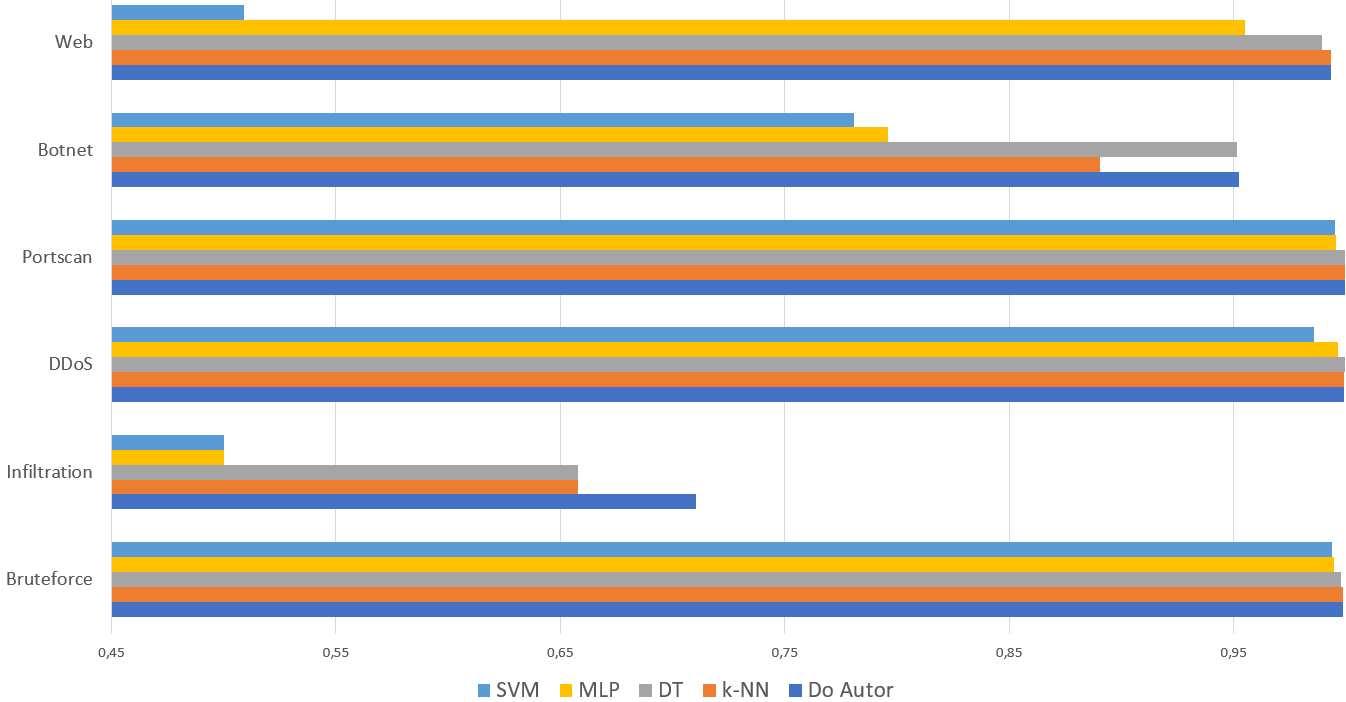
\includegraphics[width=\textwidth,keepaspectratio]{figs/mehores_resultados_defesa.png}
\newline \centering{ Fonte: Elaborado pelo autor.}\label{fig:melhores_resultados_dfesa}
\end{figure}



No Capítulo \ref{conclusoes} são apresentadas as considerações finais acerca dos resultados obtidos bem como uma análise a respeito dos  métodos utilizados na elaboração da presente Disertação de Mestrado, além da apresentação de sugestões de pesquisas futuras. 


